\documentclass[9pt]{beamer}
\usepackage{amsmath}
\usepackage{mathtext}
\usepackage{indentfirst}
\usepackage{pgf}
\usepackage{tabularx}
\usepackage{tikz}
\usepackage{gnuplot-lua-tikz}


\usetheme{Darmstadt}

\logo{\pgfputat{\pgfxy(-12.0,-0.7)}
{\pgfbox[center,base]
{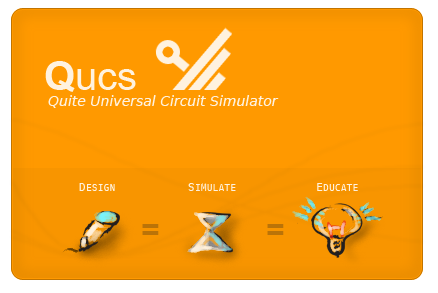
\includegraphics[width=1.3cm]{img/Qucs-logo.png}}}}

% \addtolength{\oddsidemargin}{-1cm}

\setbeamerfont{page number in head/foot}{size=\large}
\beamertemplatenavigationsymbolsempty
\setbeamertemplate{footline}[frame number]

\begin{document}


\usetikzlibrary{patterns}
\usetikzlibrary{circuits}
\usetikzlibrary{circuits.ee}
\usetikzlibrary{circuits.ee.IEC} 
\usetikzlibrary{decorations.pathmorphing,patterns}

\begin{frame}

\title{Qucs: An introduction to the new simulation and compact device modelling 
features implemented in release 0.0.19 of the popular GPL circuit simulator}

\author{ \small
Mike Brinson \inst{1}, \url{mbrin72043@yahoo.co.uk.} \\ \and 
Richard Crozier \inst{2},  \url{richard.crozier@yahoo.co.uk} \\ \and 
Vadim Kuznetsov \inst{3}, \url{ra3xdh@gmail.com} \\ \and 
Clemens Novak \inst{4}, \url{clemens@familie-novak.net} \\ \and 
Bastien Roucaries \inst{5}, \url{bastien.roucaries@satie.ens-cauchan.fr} \\ 
\and Frans Schreuder \inst{6}, \url{fransschreuder@gmail.com} \\ \and 
Guilherme Brondani Torri \inst{4}, \url{guitorri@gmail.com} }

\institute{
\inst{1} Centre for Communications Technology, London Metropolitan 
 University, UK \and
\inst{2} The University of Edinburgh, UK \and
\inst{3} Bauman Moscow Technical University, Russia \and
\inst{4} Qucs Developer \and 
\inst{5}  Laboratoire SATIE --- CNRS UMR 8929, Universit\'{e}  de 
Cergy-Pontoise, ENS Cachan, FR \and
\inst{6} Nikhef, Amsterdam, NL }

\maketitle

\end{frame}

\begin{frame}
 \frametitle{Qucs: An introduction to the new simulation and compact device 
modelling features implemented in release 0.0.19 of the popular GPL circuit 
simulator}
\small

\begin{itemize}
 \item Future Qucs structure overview
 \item Spice4qucs initative tasks and main features
 \item Ngspice and Xyce applications for Qucs circuits simulation: 
legacy Qucs circuits simulation, realistic circuits, power electronics. 
Qucs2spice netlist converter.
 \item Compact modelling with Qucs, Ngspice, and Xyce
 \begin{itemize}
  \item EDD support: Current and charge equations
  \item XSCPICE macromodels support
  \item B-type sources
  \item Harmonic balance simulation with Xyce and Qucs compact models
  \item Capacitance measurement with Ngspice and Qucs
 \end{itemize}
 \item {New components coming with Spice4qucs overview }
 \begin{itemize}
  \item Behavioral and modulated sources: B-type, PWL, AM, SFFM
  \item Transmission lines: TLINE, LTRA, UDRCTL, noise
  \item Full SPICE semiconductor devices: Diode, BJT, JFET, MOSFET, MESFET
 \end{itemize}
  \item Parametrization features of Spice4qucs and Ngnutmeg scripting
  \item New Analysis types from Spice4qucs (.FOUR, .NOISE, .DISTO)
  \item Ngspice "Custom simulation" technique
  \item New tools for active and passive filter synthesis
  \item Plans for future



\end{itemize}


\end{frame}

\begin{frame}
 \frametitle{Future structure of Qucs}
%  \hspace{-10mm}
 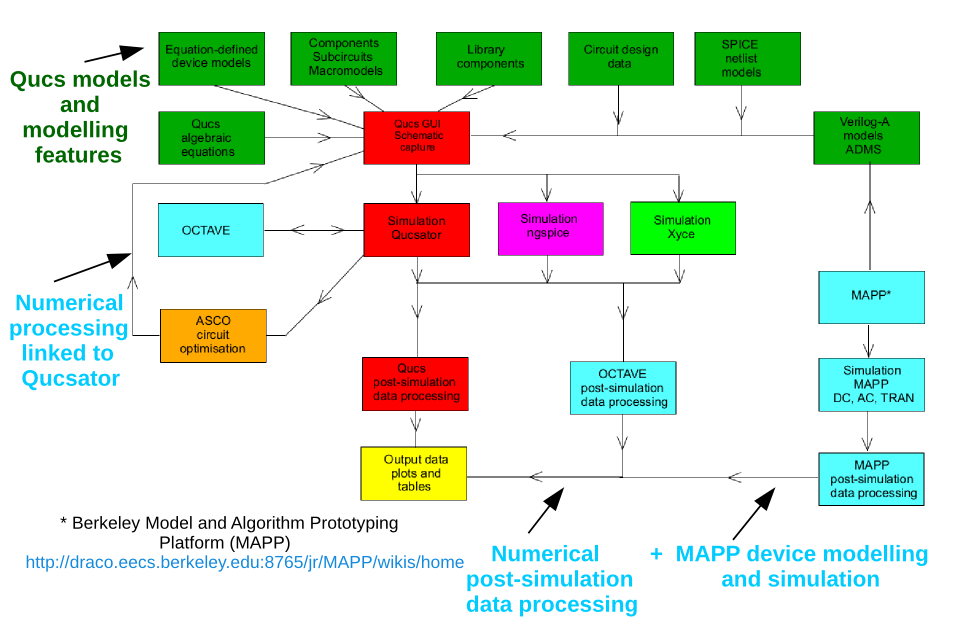
\includegraphics[width=\textwidth]{img/Spice4qucsFig2.png}
\end{frame}


\begin{frame}
 \frametitle{Overview of spice4qucs structure: Part I --- spice4qucs initiative 
tasks}
 
%  \hspace{-1.2cm}
  \begin{tabular}{p{0.4\textwidth}p{0.6\textwidth}}
  \tiny
  Spice4qucs initative tasks:
  
   \begin{itemize}
    \item Correct known weaknesses observed with the current Qucs simulation 
engine qucsator .
    \item Provide Qucs users with a choice of simulator selected from 
qucsator, ngspice and Xyce. 
    \item Extend Qucs subcircuit, EDD, RFEDD and Verilog-A device modelling 
capabilities.
    \item Access to the additional simulation tools and extra 
component and device models provided by ngspice and Xyce. 
    \item Mixed-mode analogue-digital 
circuit simulation capability using Qucs/ngspice/XSPICE simulation.
   \end{itemize}
   
   Currently implemnted in Qucs-0.0.19:
   
   \begin{itemize}
    \item Ngspice, Xyce (both serial and parallel) support
    \item Basic simulations support (.DC, .AC, .TRAN)
    \item Advanced simulation support (.FOUR, .DISTO, .NOISE, .HB)
    \item Semiconductor devices with full SPICE definition
    \item Qucs equations, parametrization (.PARAM), and Ngnutmeg scripts support
    \item Custom Ngspice simulation technique --- User ngnutmeg simulation 
    scripts support.
   \end{itemize}

  
  &    \tiny 
     \begin{itemize}
      \item  Qucs$<$---$>$Ngspice/Xyce interfacing schematic
     \end{itemize}
     
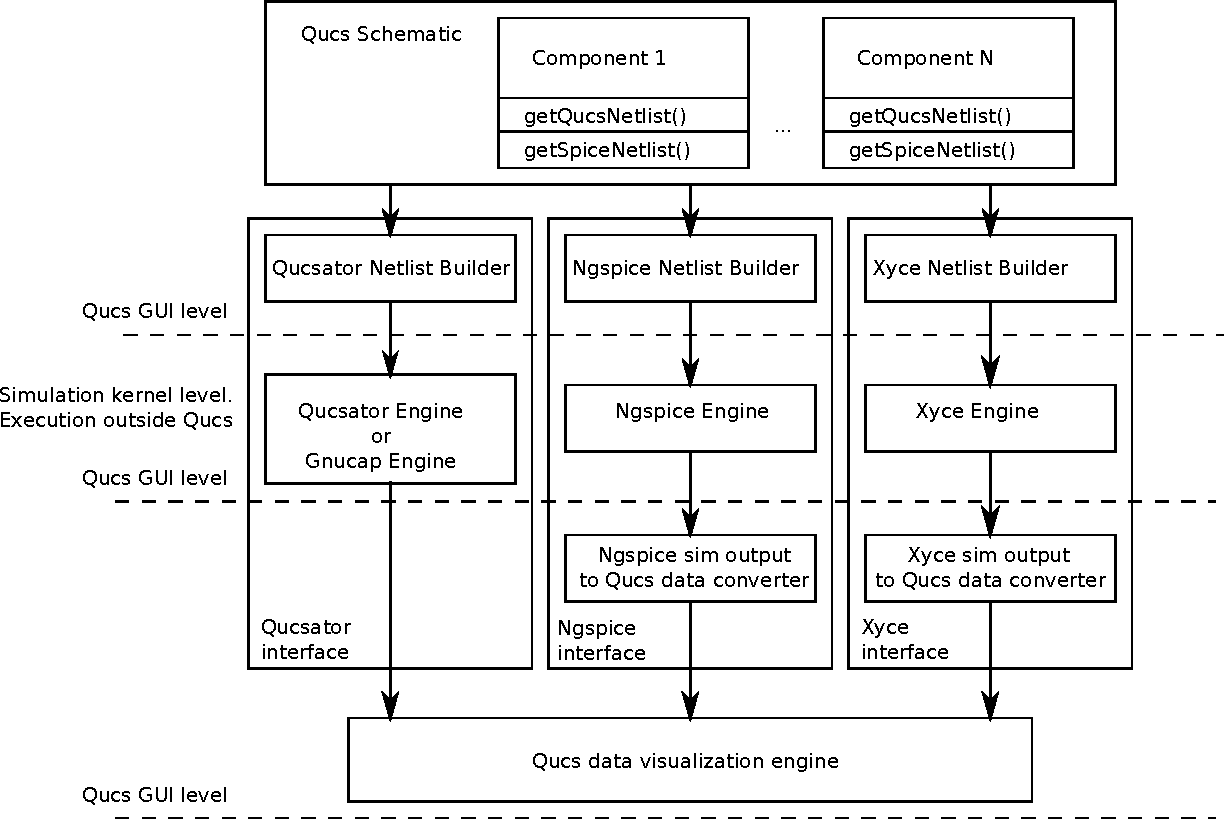
\includegraphics[width=0.65\textwidth]{img/spice4qucs.pdf} 
     \begin{itemize}
      \item Spice4qucs online documentation available here: 
\url{https://qucs-help.readthedocs.org/en/spice4qucs/index.html}
     \end{itemize} \\

  
  \end{tabular} 

 
\end{frame}

\begin{frame}
 \frametitle{Overview of spice4qucs structure: Part II --- New features coming 
with Spice4qucs}
  \begin{tabular}{p{0.5\textwidth}p{0.5\textwidth}}
  
  The list of supported simulations:
    \begin{itemize}
     \item Qucsator, Ngspice, and Xyce:
     \begin{itemize}
      \item DC sweep analysis
      \item AC small signal analysis
      \item Transient analysis
      \item Single parameter sweep
     \end{itemize}
     \item Qucsator and Ngspice: Parameter sweep in nested loops
     \item Qucscator and Xyce only: Harmonic balance (HB)
     \item Ngspice and Xyce: Fourier analysis
     \item Ngspice only:
     \begin{itemize}
      \item Distortion analysis
      \item Noise analysis
      \item Custom simulation --- Ngnutmeg script embedded in Qucs schematic
     \end{itemize}

    \end{itemize}
    & New "SPICE simulation" dialog
    
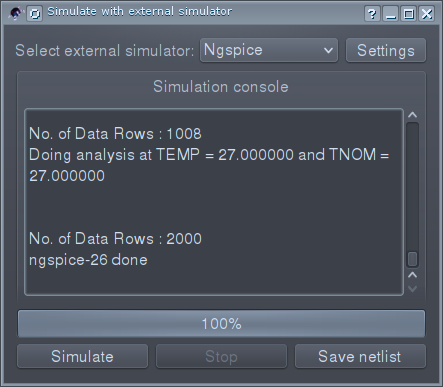
\includegraphics[width=0.5\textwidth]{img/s4q_dlg.png} \\
  \end{tabular}

\end{frame}


\begin{frame}
 \frametitle{Ngspice and Xyce simulation techniques: Part I --- Legacy Qucs 
circuit simulated with Ngspice and Xyce}
\pgfputat{\pgfxy(-1.0,-4.3)}
{\pgfbox[bottom,base]
{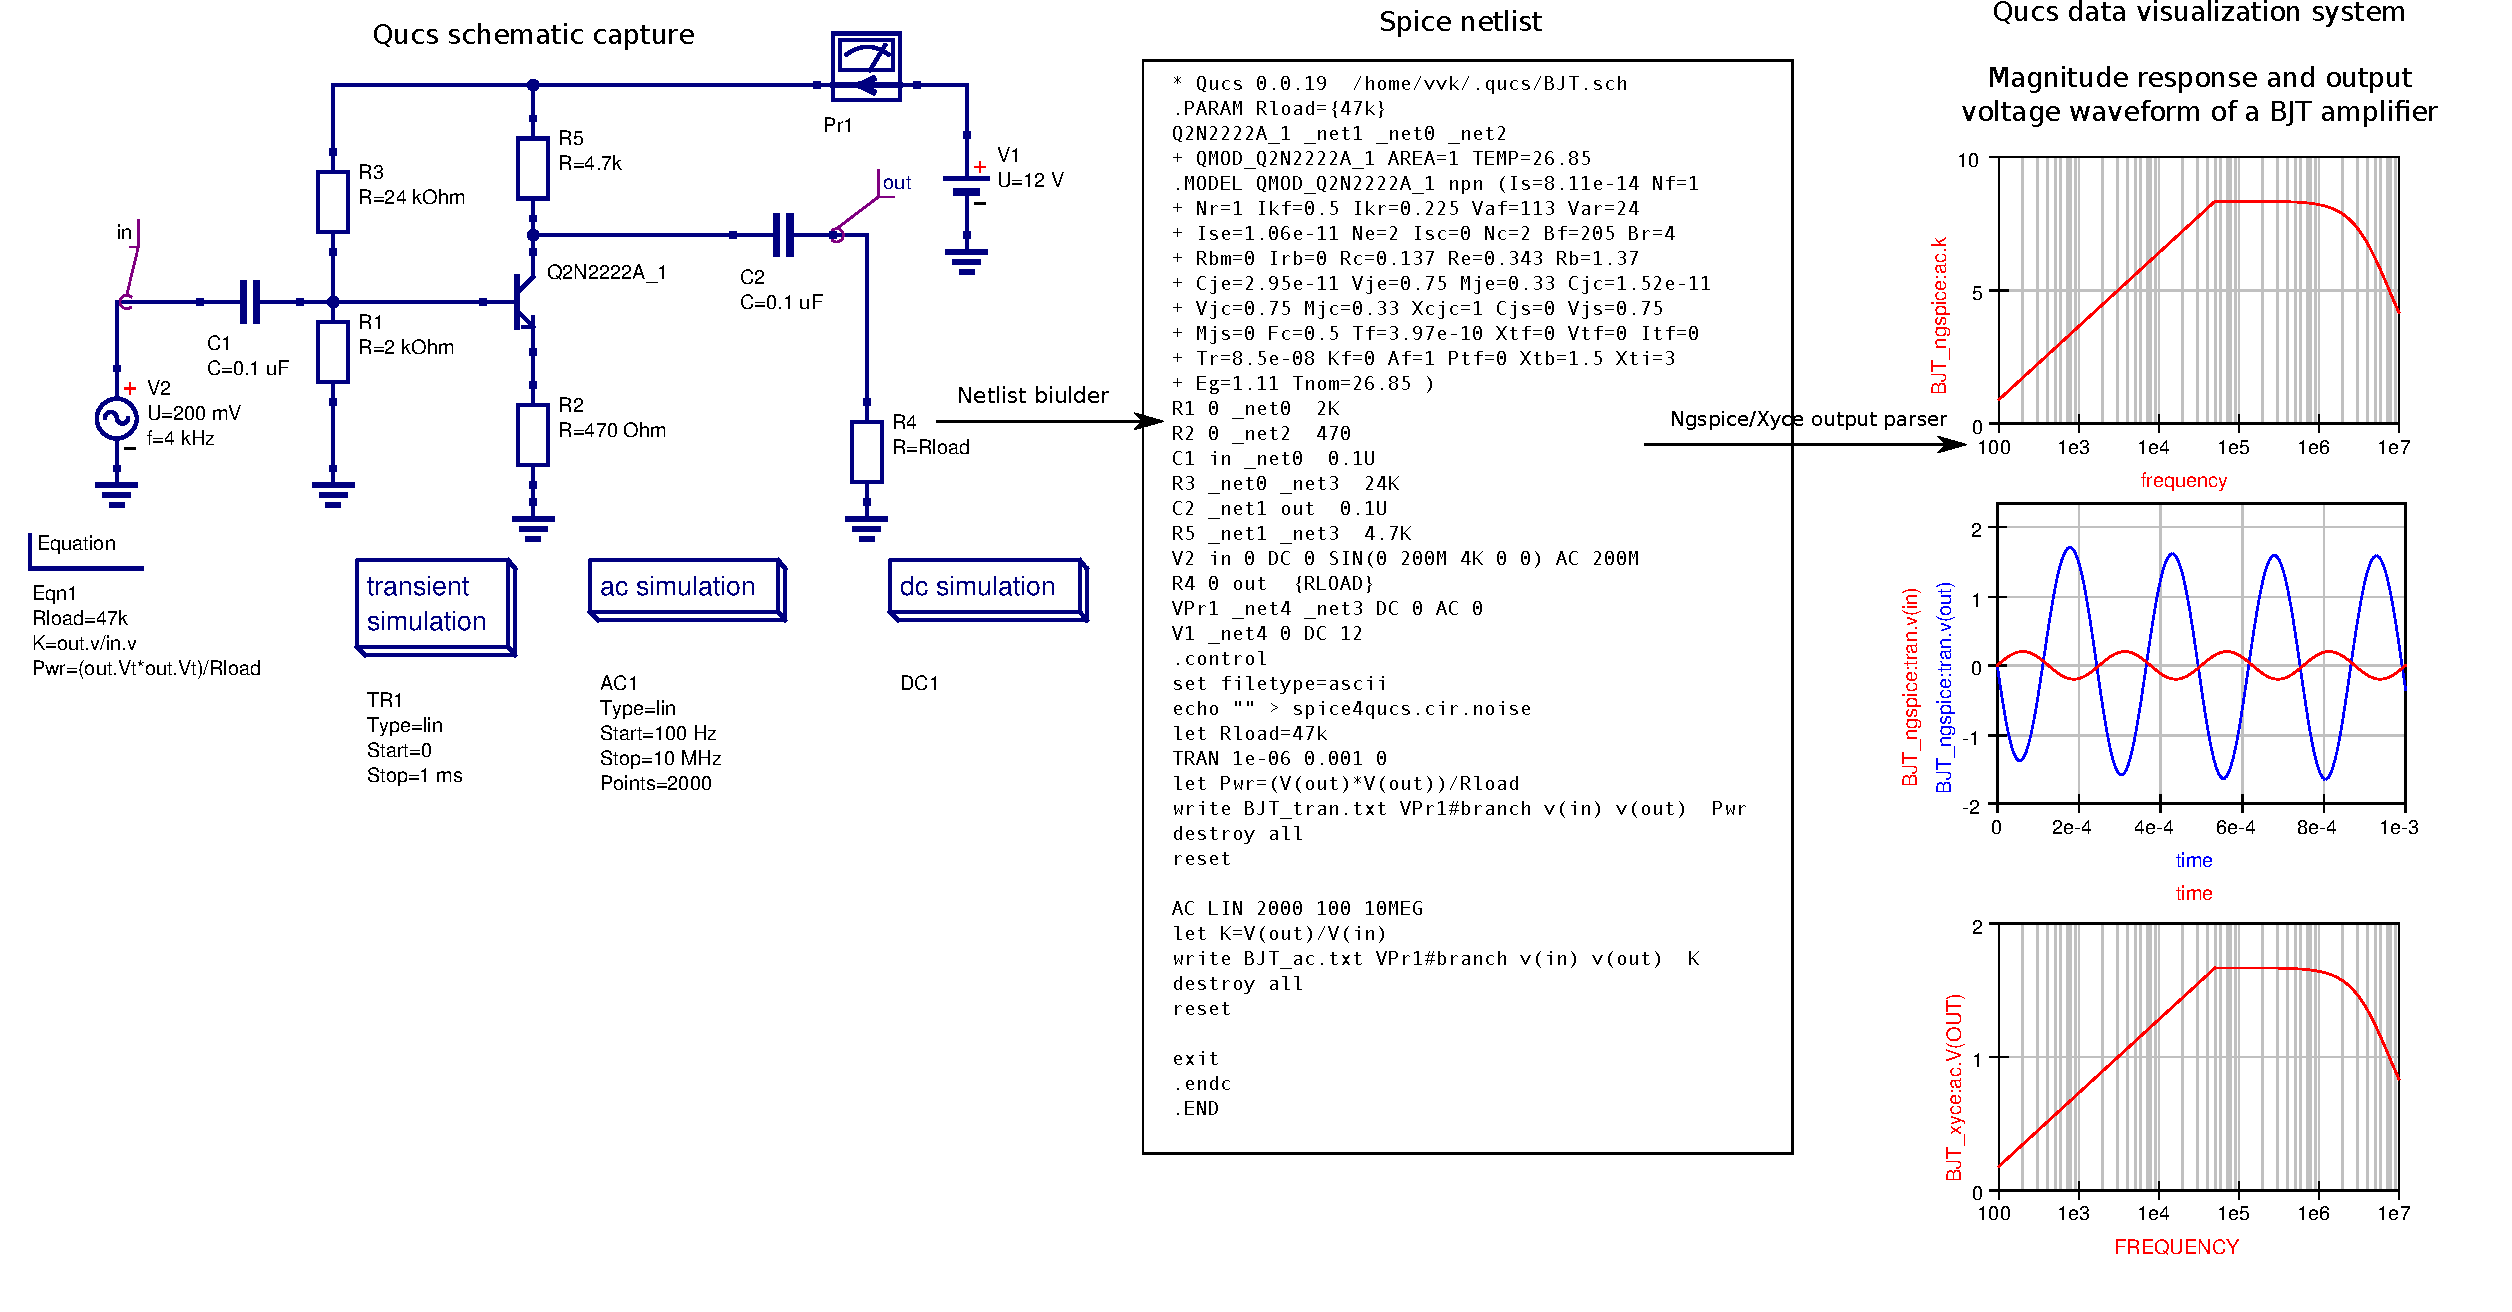
\includegraphics[width=1.2\textwidth]{img/BJT-s4q.pdf}}}


\end{frame}


\begin{frame}
 \frametitle{Ngspice and Xyce simulation techniques: Part II --- Realistic 
circuits simulation with Ngspice and Xyce}
This example shows realistic circuit simulation technique with Ngspice. BJT 
audio amplifier is simulated in both frequency and time domain.

 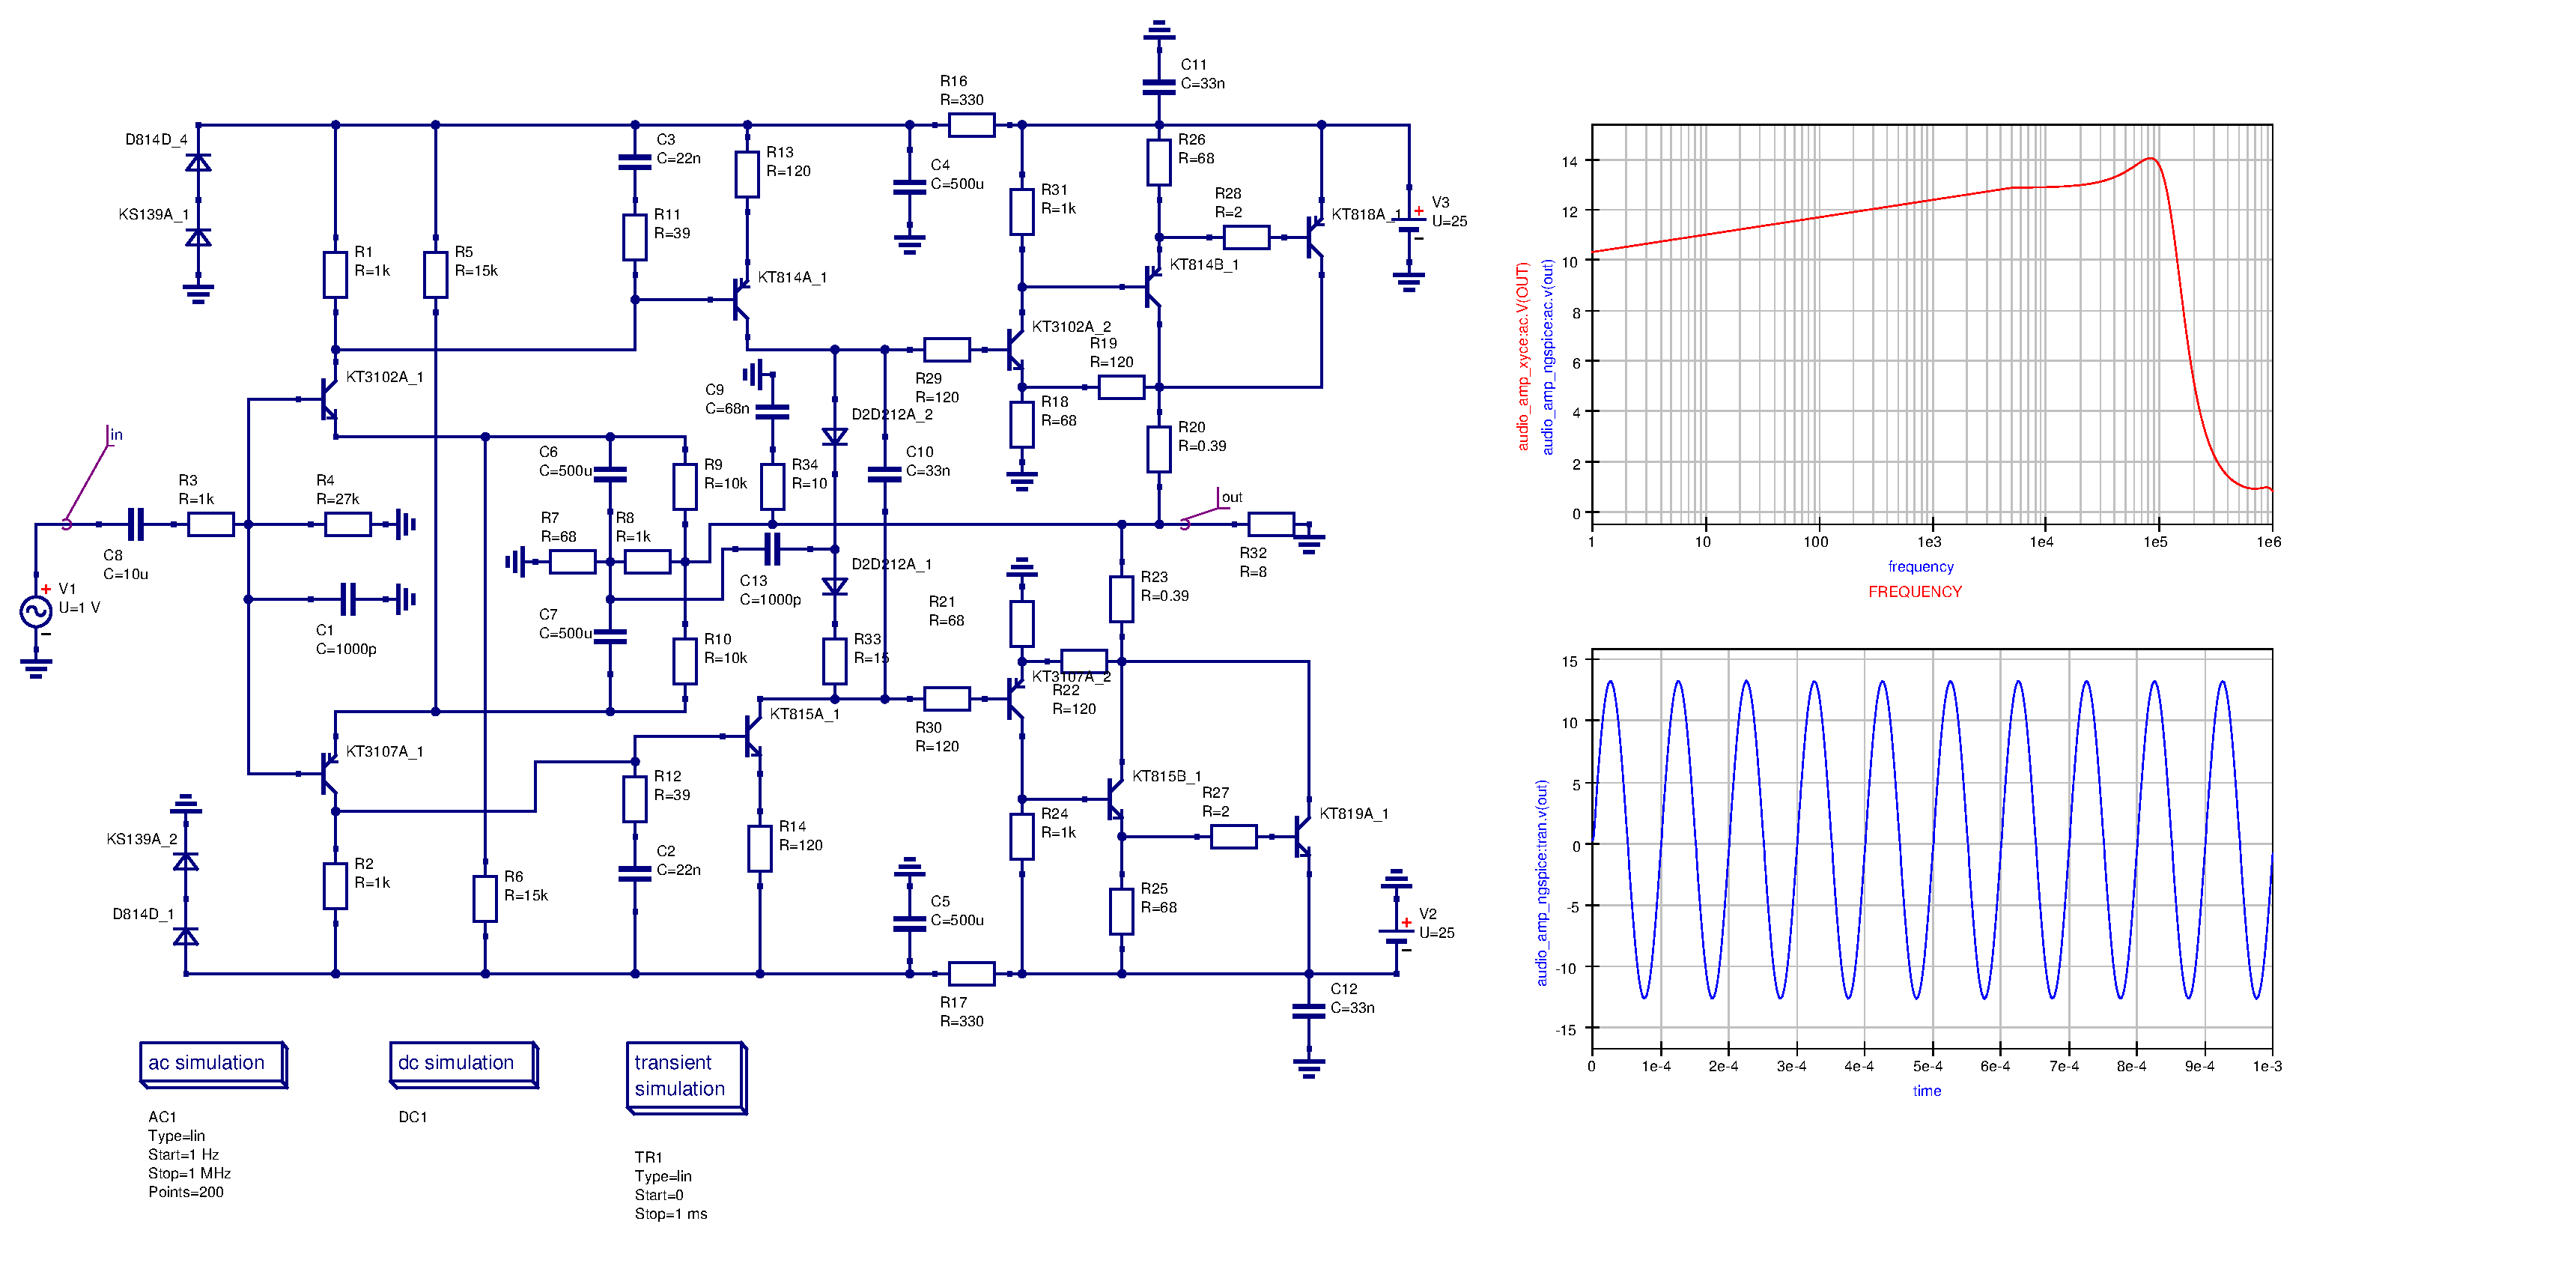
\includegraphics[width=1.1\textwidth]{img/au_amp.pdf}
\end{frame}

\begin{frame}
 \frametitle{Ngspice and Xyce simulation techniques: Part III --- Power 
electronics simulation with Ngspice and Xyce}

\begin{itemize}
 \item MOSFET switch with inductive load simulation with Ngspice and Xyce.  
This example shows Qucs library components support with spice4qucs
 \item SPICE model of MOSFET is converted from Qucs library model using 
qucs2spice subsystem
\end{itemize}

 

 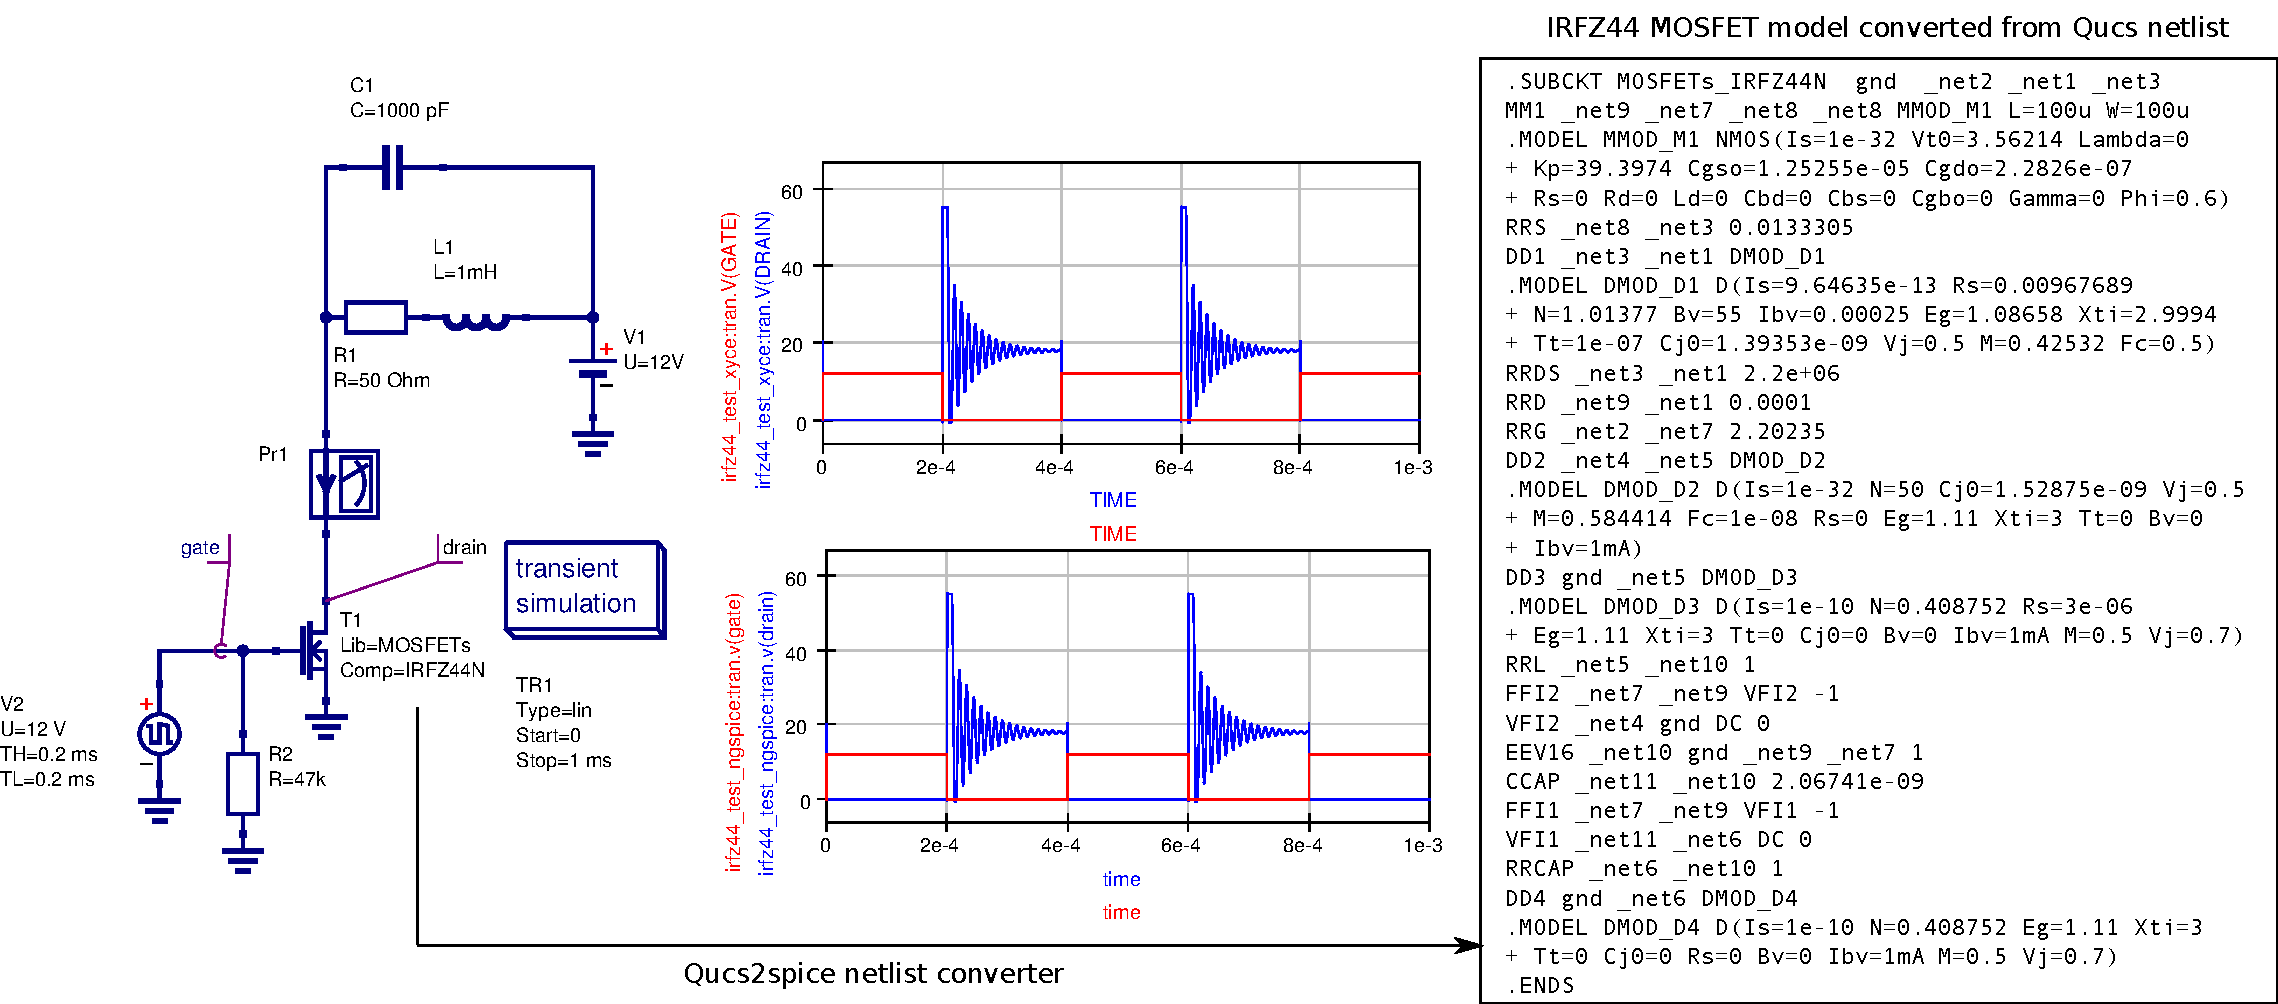
\includegraphics[width=1\textwidth]{img/irfz44.pdf}
 

\end{frame}


\begin{frame}
 \frametitle{Compact modeling with Qucs and Ngspice/Xyce: Part I --- Current 
equations support}

Let's consider tunnel diode model:

\begin{equation}
 I = I_s\left(e^{\frac{V}{\varphi_T}}-1\right) + I_ve^{k(V-V_v)} + 
     I_p\cdot\frac{V}{V_p}e^{\frac{V_p-V}{V_p}} \label{eq:tun}
\end{equation}

Current equations in Qucs EDDs could be represented with B-type Ngspice/Xyce 
current sources:

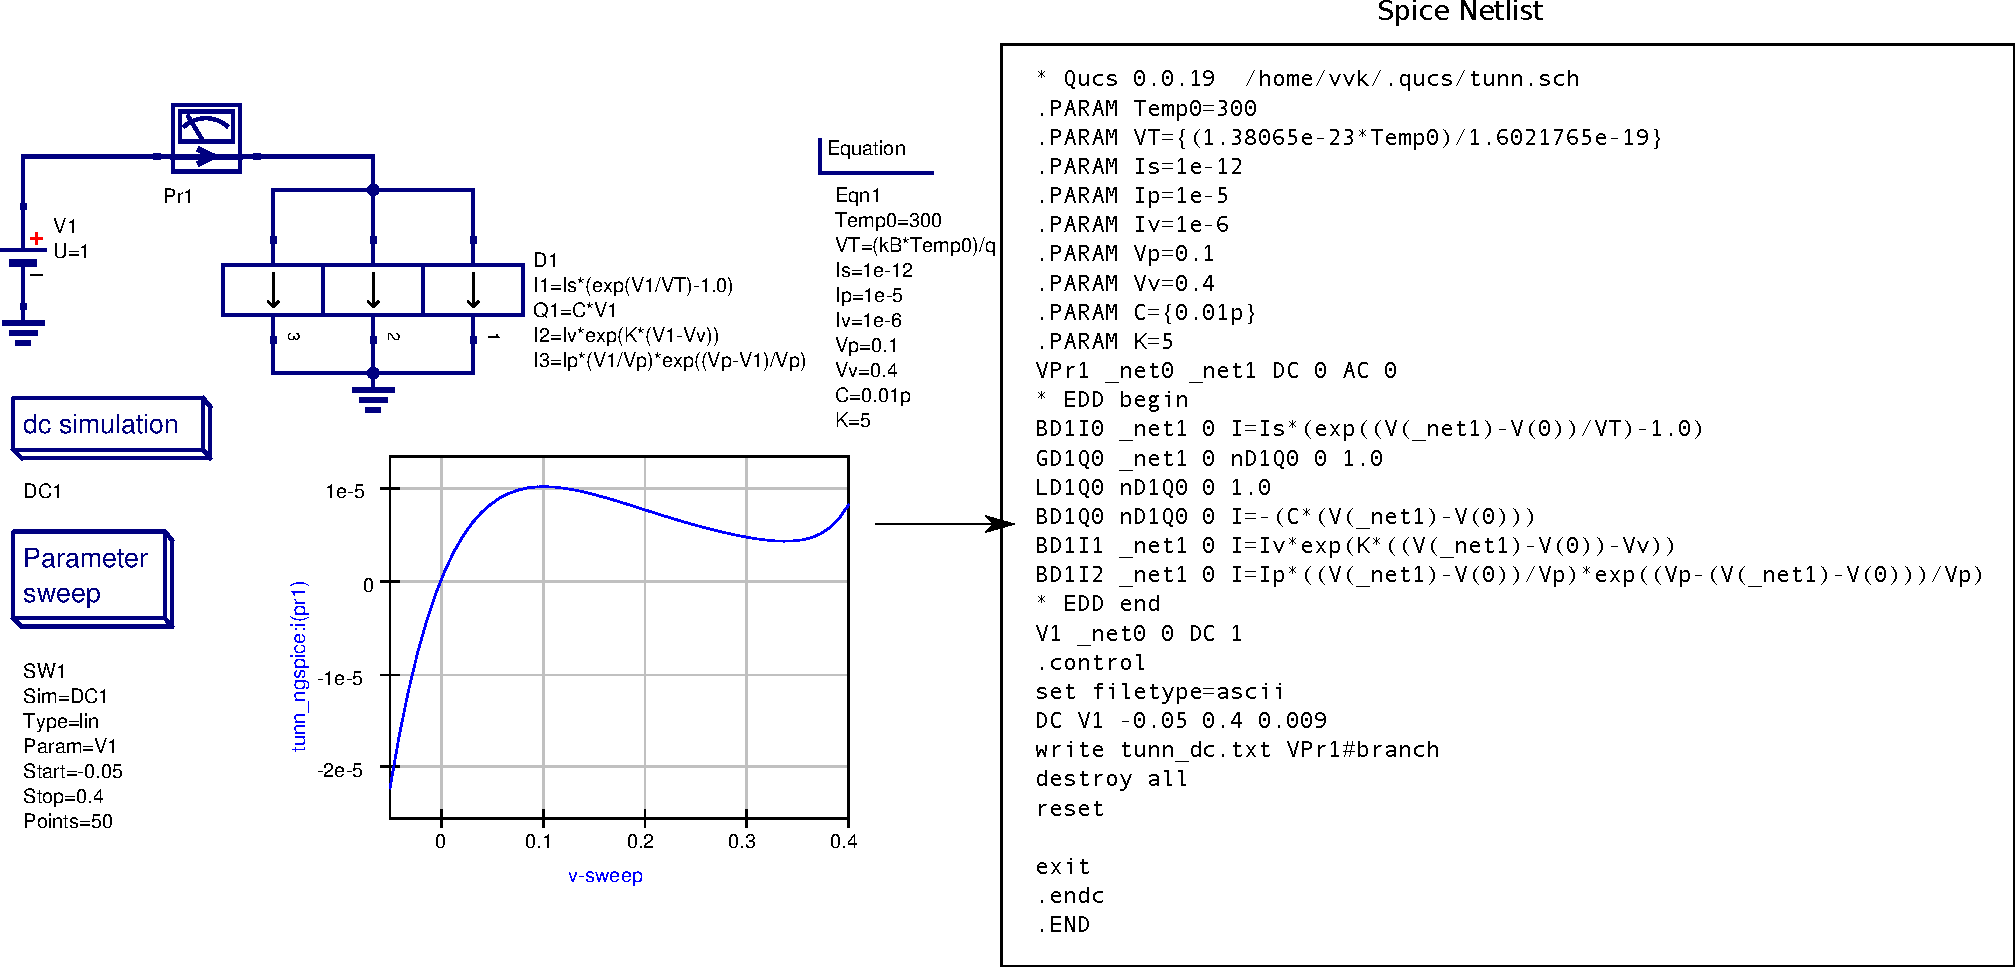
\includegraphics[width=0.9\textwidth]{img/tunn.pdf}

\end{frame}

\begin{frame}
 \frametitle{Compact modeling with Qucs and Ngspice/Xyce: Part II --- Charge 
equations approach}

\hspace{-1cm}
  \begin{tabular}{p{0.3\textwidth}p{0.7\textwidth}}
  
  Current and voltage on nonlinear capacitance:
  \begin{equation}
   I = \frac{dQ}{dt} =\frac{d}{dt} C V
  \end{equation}
  
  Xyce and Ngspice has no support of diff() operator. It's need to use 
 equivalent circuit approach to represent charge equations.
 
   & 
\begin{itemize}
 \item Nonlinear capacitance equivalent circuit 
\end{itemize}

 
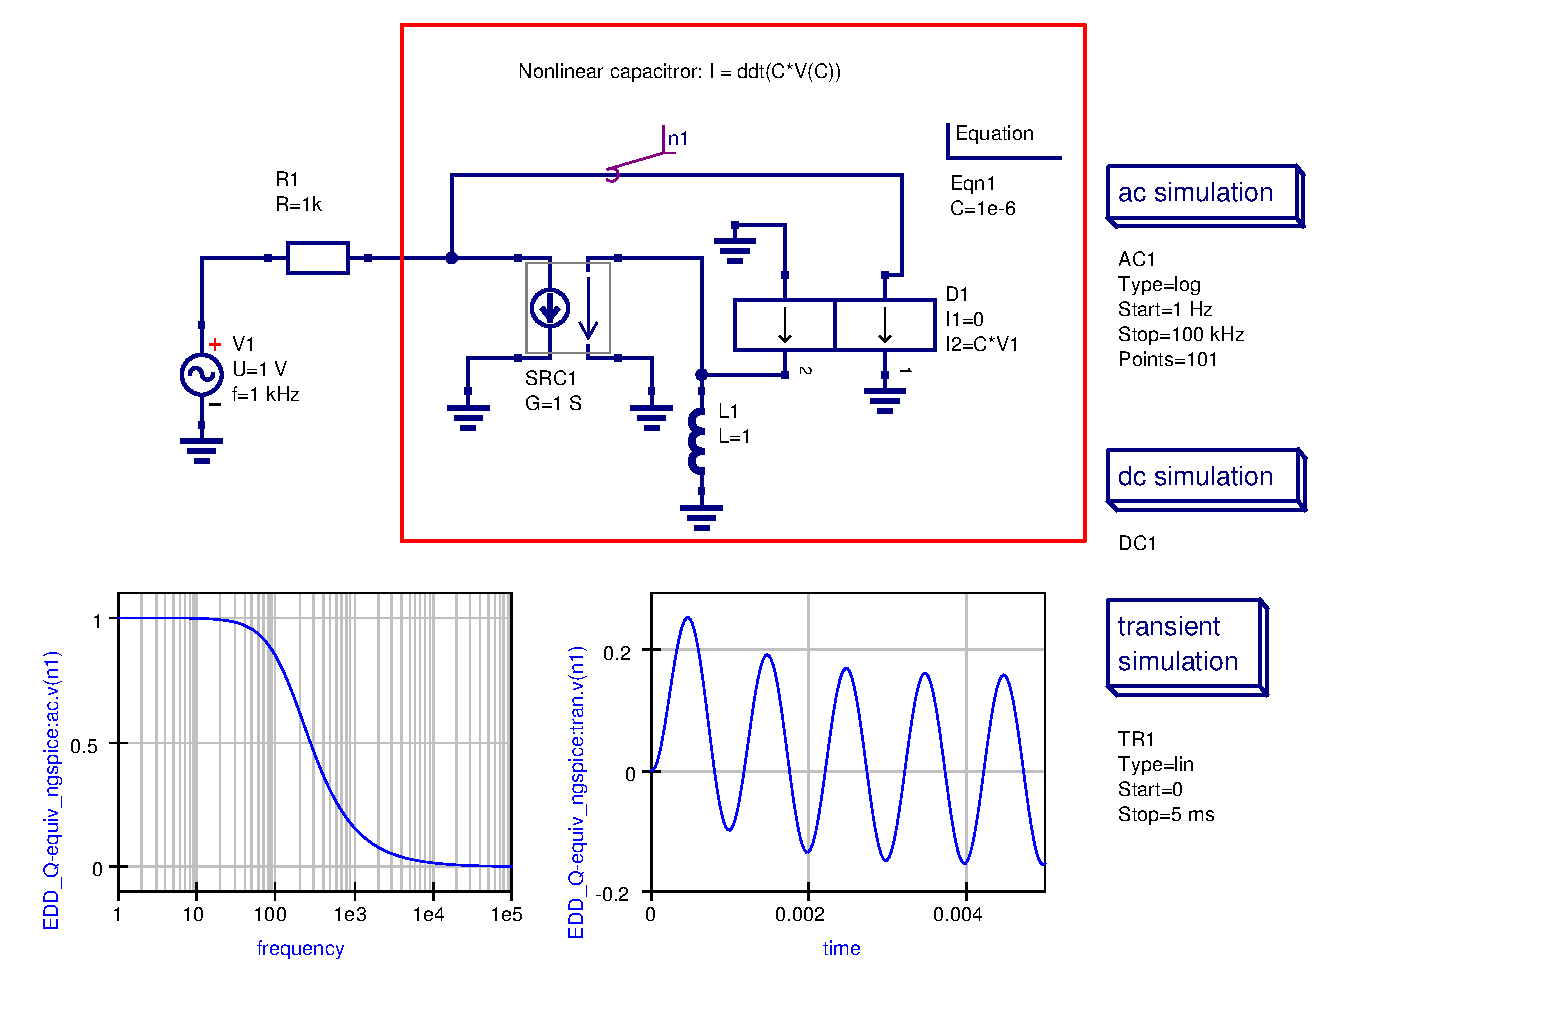
\includegraphics[width=0.9\textwidth]{img/Cap-equiv.pdf} \\
  \end{tabular}

 \end{frame}
 
 \begin{frame}
  \frametitle{Compact modeling with Qucs and Ngspice/Xyce: Part III --- Charge 
equations usage example}

\begin{itemize}
 \item Let's simulate nonlinear capacitance with Ngspice and Xyce:
 \begin{equation}
 Q = C_1V + \frac{C_2V^2}{2} + \frac{C_3V^3}{3} + \ldots + \frac{C_NV^N}{N}
\end{equation}
\end{itemize}

 


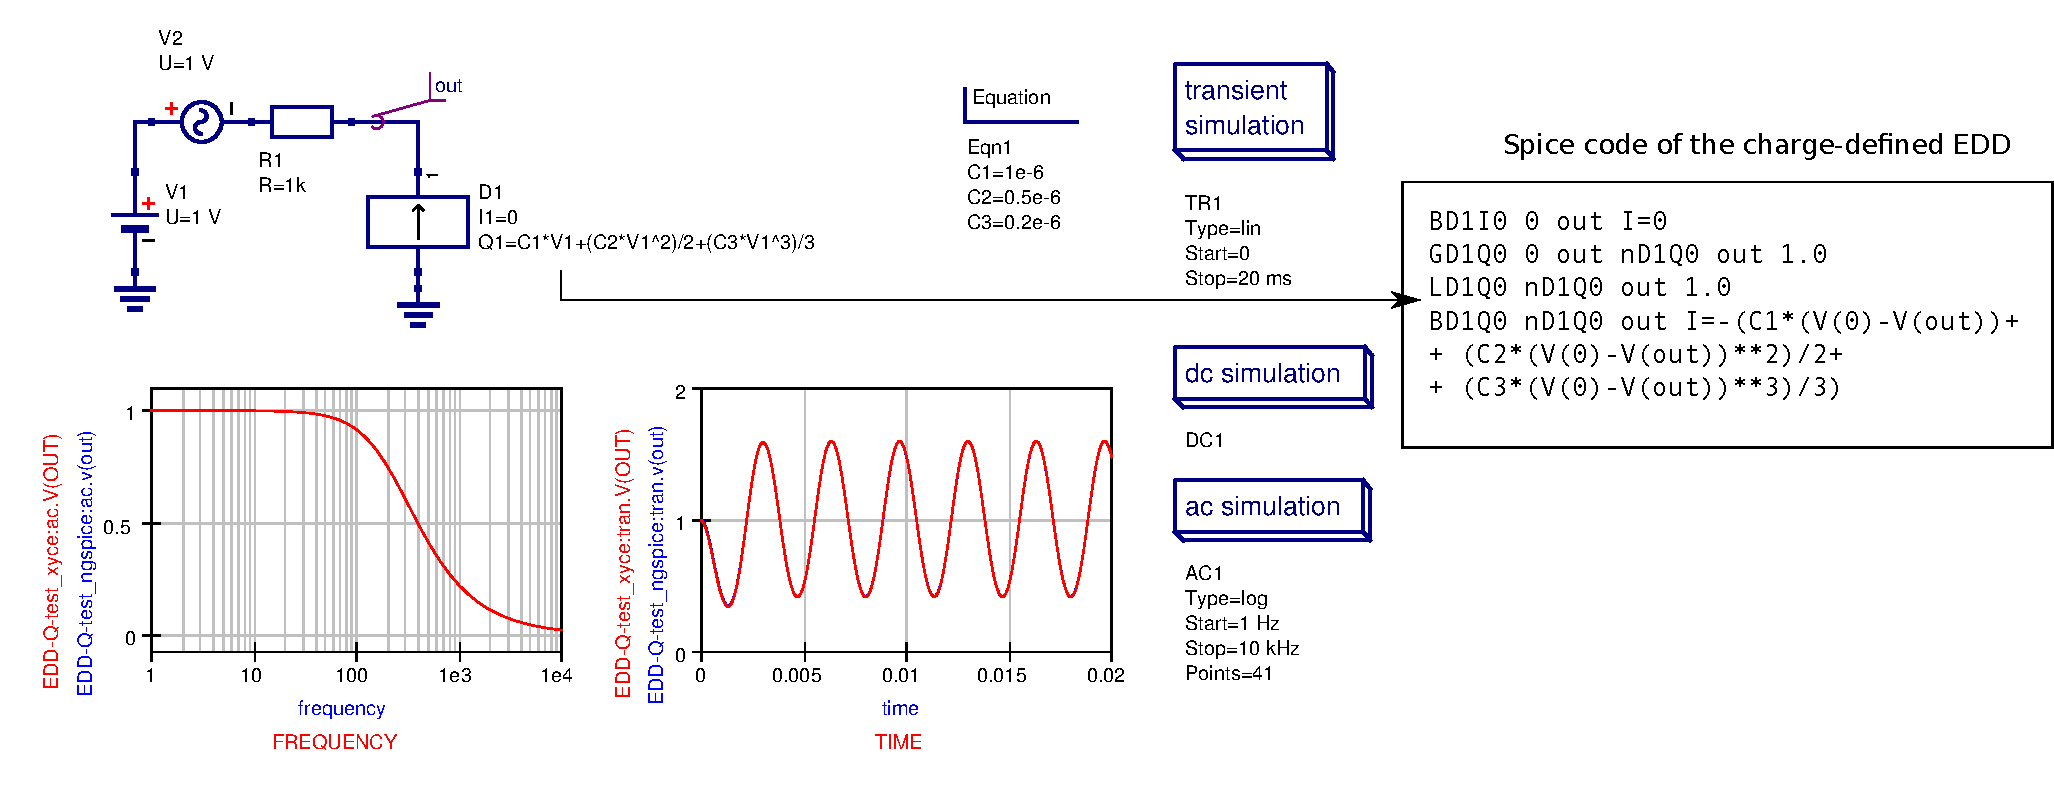
\includegraphics[width=1.05\textwidth]{img/CapTest.pdf}

 \end{frame}

 \begin{frame}
    \frametitle{Compact modeling with Qucs and Ngspice/Xyce: Part IV --- 
B-type source usage for compact modeling}

\begin{itemize}
 \item Qucs 0.0.19 introduces a new component: SPICE-compatible equation 
defined voltage or current source (B-type source). You can easily build compact 
models with it.
\end{itemize}


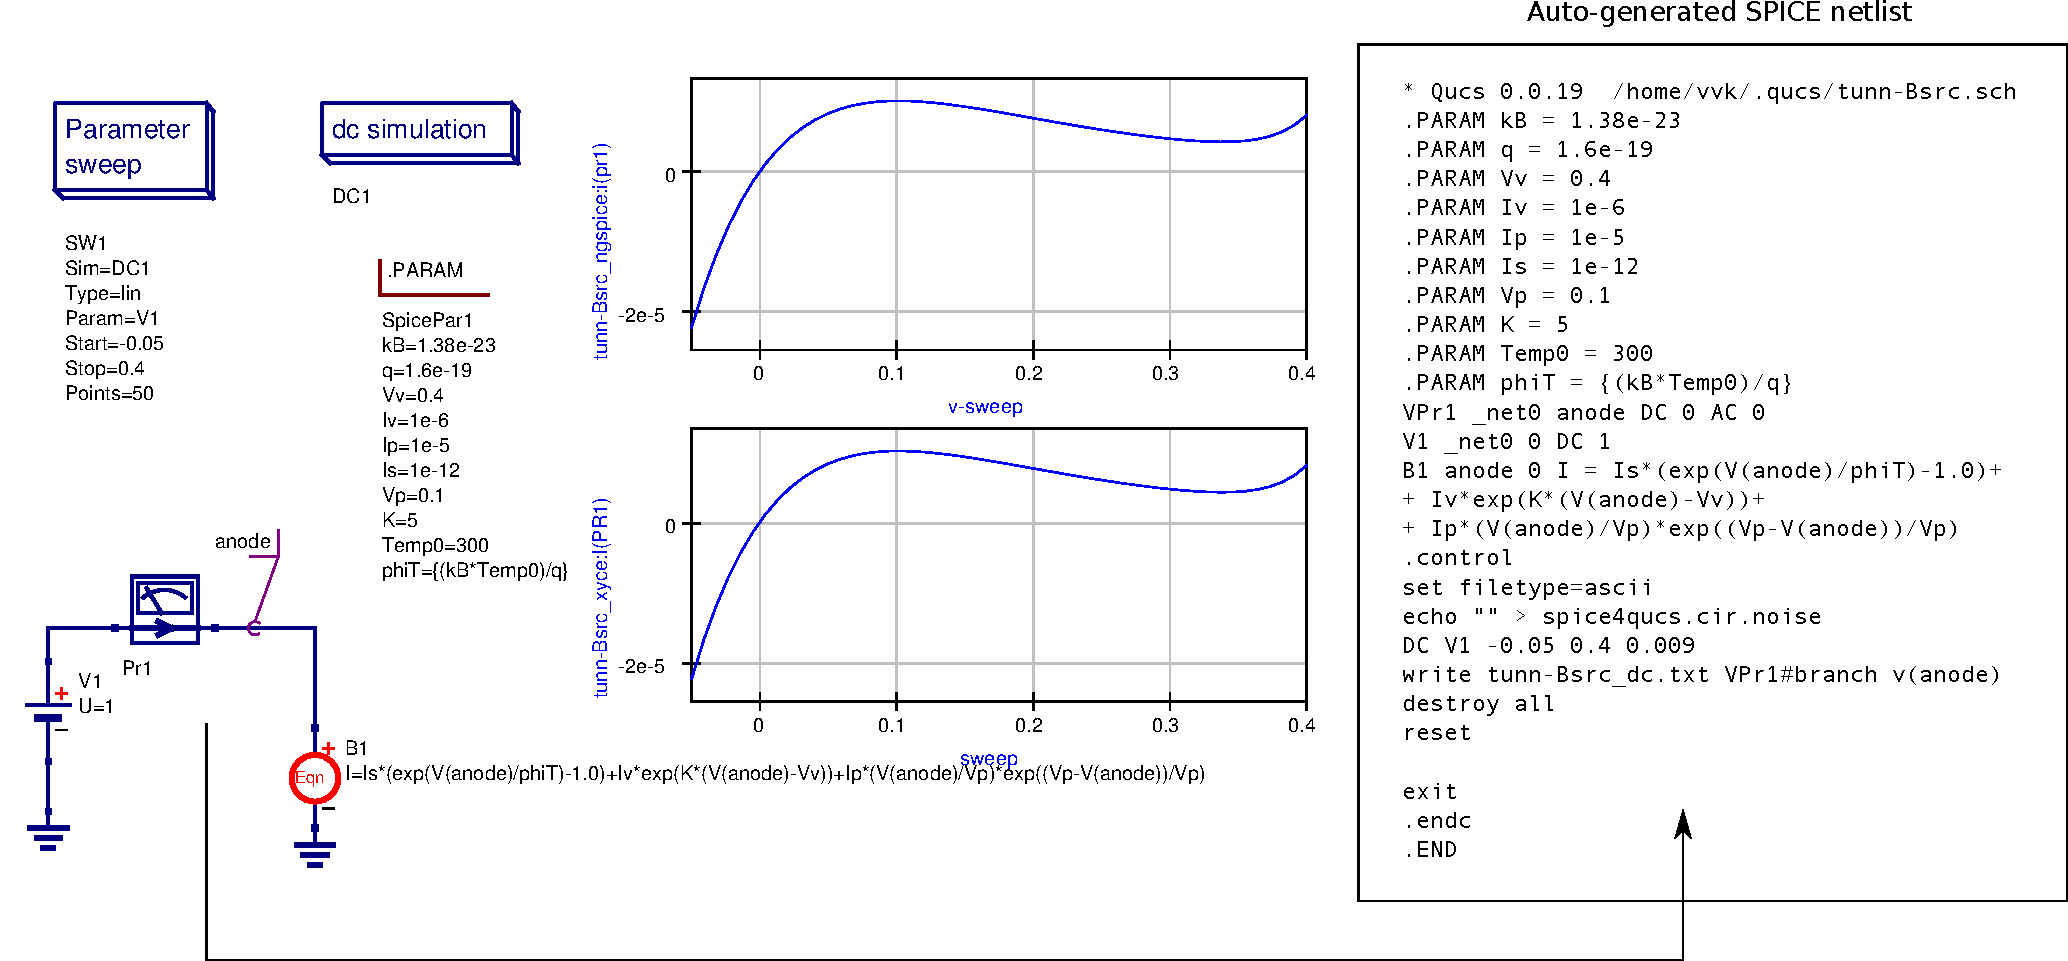
\includegraphics[width=1.05\textwidth]{img/tunn-Bsrc.pdf}


 \end{frame}

 
  \begin{frame}
    \frametitle{Compact modeling with Qucs and Ngspice/Xyce: Part V --- 
NPN BJT compact model used for Harmonic balance analysis of one-stage BJT 
amplifier}

\begin{itemize}
 \item Spice4qucs and Xyce allows you to use compact model with 
Harmonic-balance analysis
 \item Subcircuit of NPN BJT using compact models
\end{itemize}

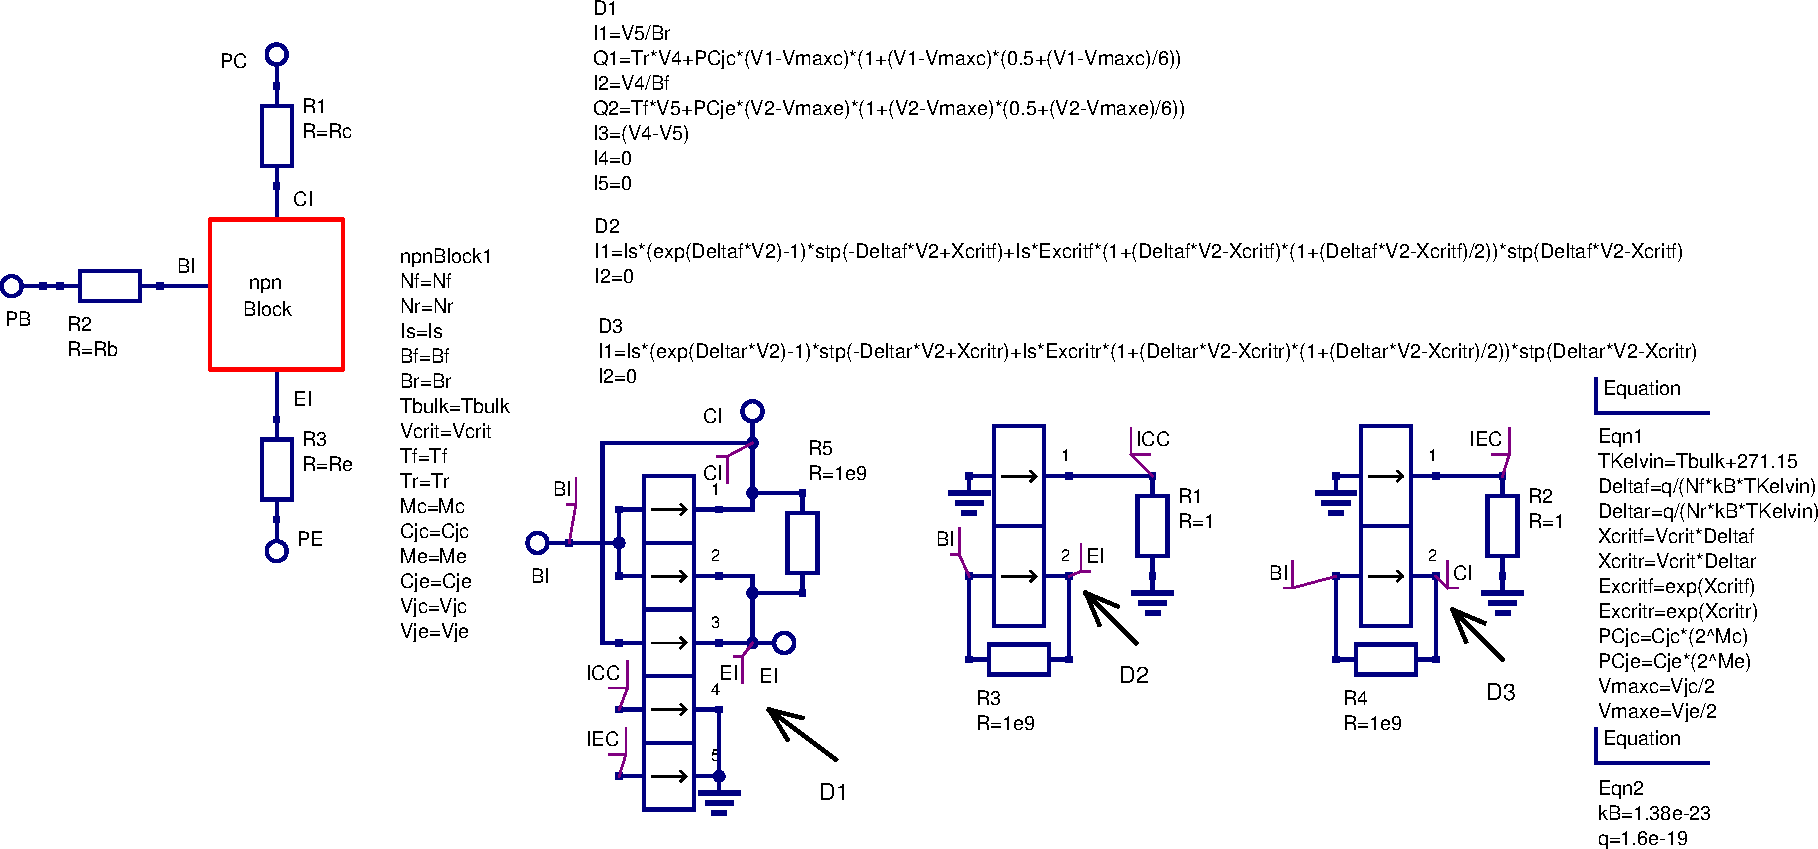
\includegraphics[width=1.05\textwidth]{img/npnBlock.pdf}


 \end{frame}
 
   \begin{frame}
    \frametitle{Compact modeling with Qucs and Ngspice/Xyce: Part VI --- 
HB analysis results and SPICE netlist of BJT amplifier}

\vspace{-2cm}
\begin{itemize}
 \item Xyce harmonic balance simulation data and auto-generated netlist for 
one-stage BJT amplifier
 \item More info at \url{Here will be hyperlink for MIXDES-2015 paper}
\end{itemize}
\vspace{3mm}

\pgfputat{\pgfxy(-0.5,-3.5)}
{\pgfbox[bottom,base]
{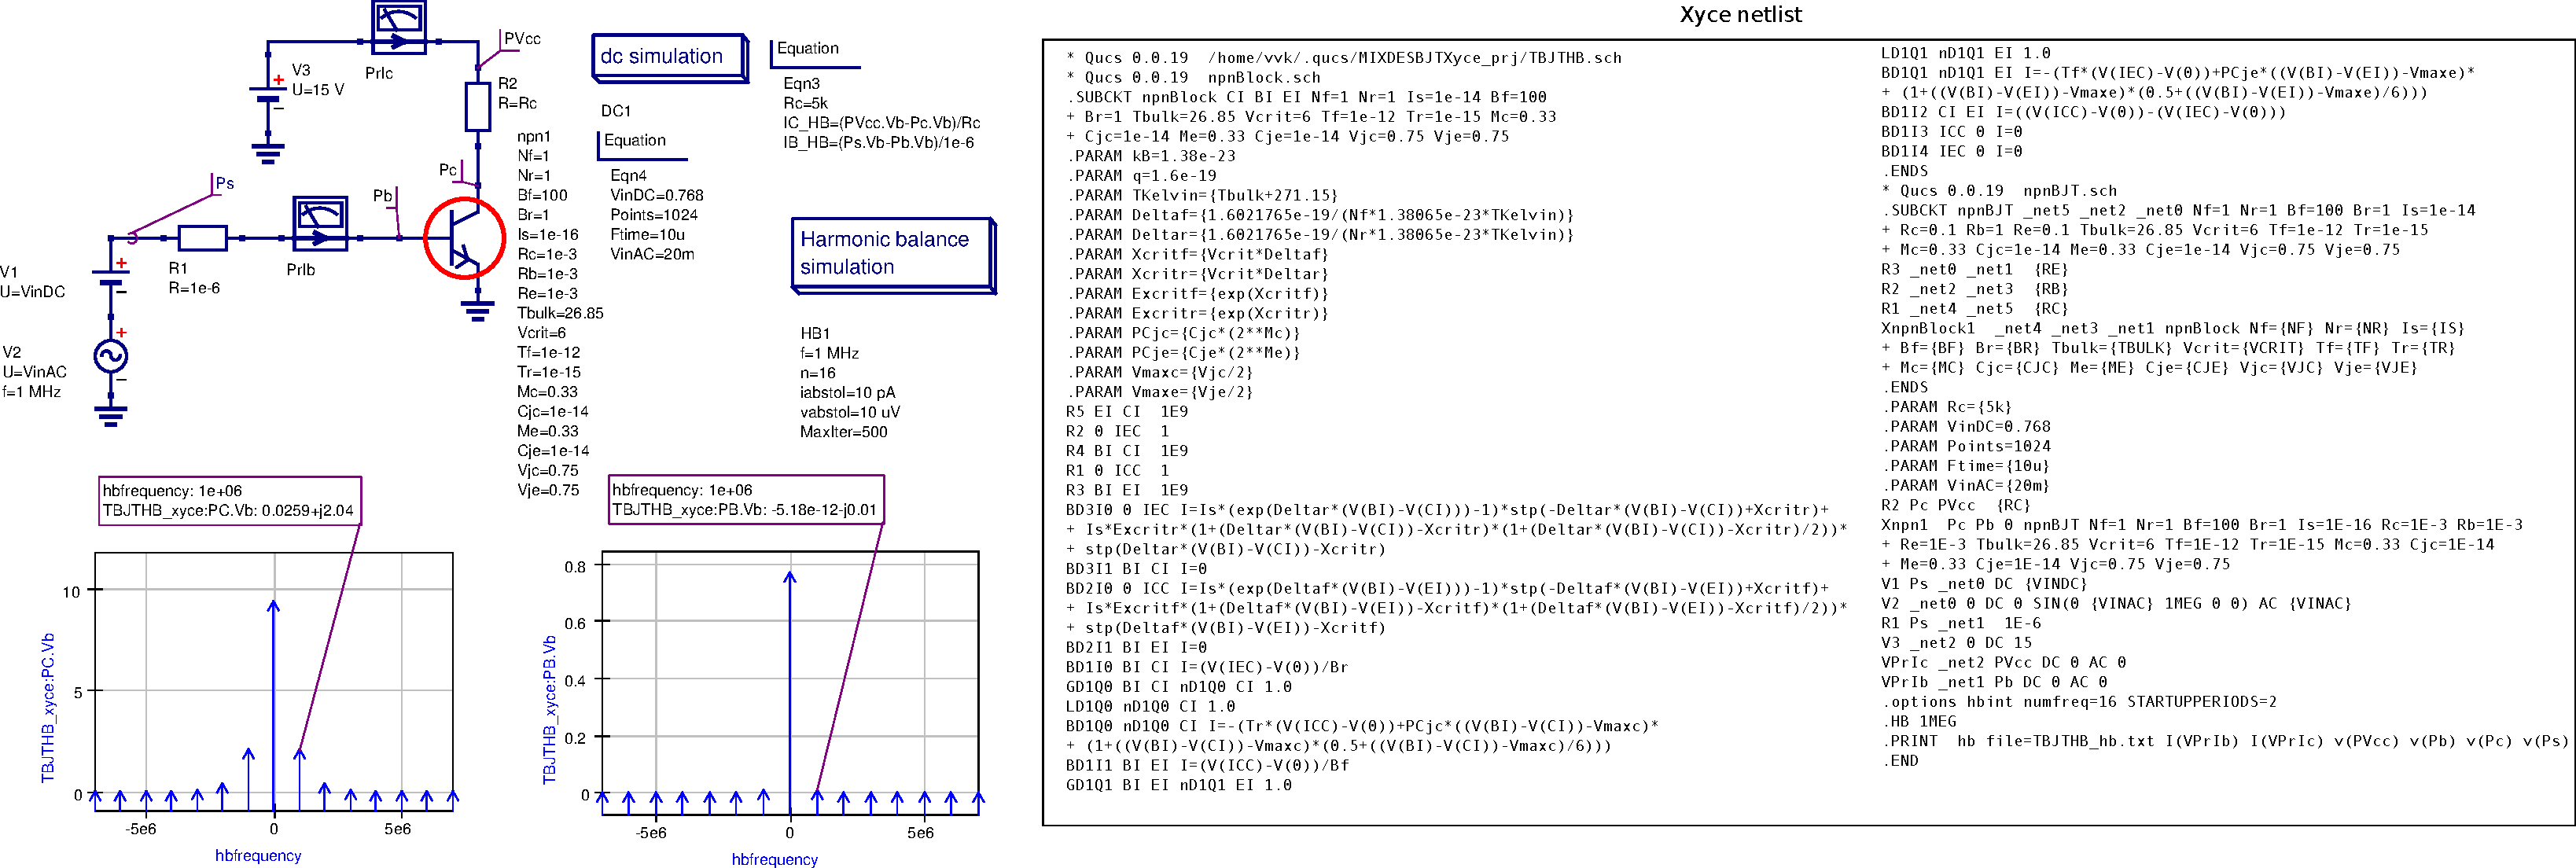
\includegraphics[width=1.1\textwidth]{img/npnHB.pdf}}}


 \end{frame}
 
 \begin{frame}
  \frametitle{Compact modeling with Qucs and Ngspice/Xyce: Part VII --- 
XSPICE macromodels usage}

 \begin{itemize}
  \item Since Qucs-0.0.19 embedding of SPICE-model in Qucs libraries is 
allowed 
  \item Applications of this feature:
  \begin{itemize}
   \item Direct simulation of SPICE-defined components
   \item XSPICE macromodels usage
  \end{itemize}
  \item{LM358 XSPICE macromodel usage example (noninverting amplifier)}
 \end{itemize}
 
 \hspace{-8mm}
 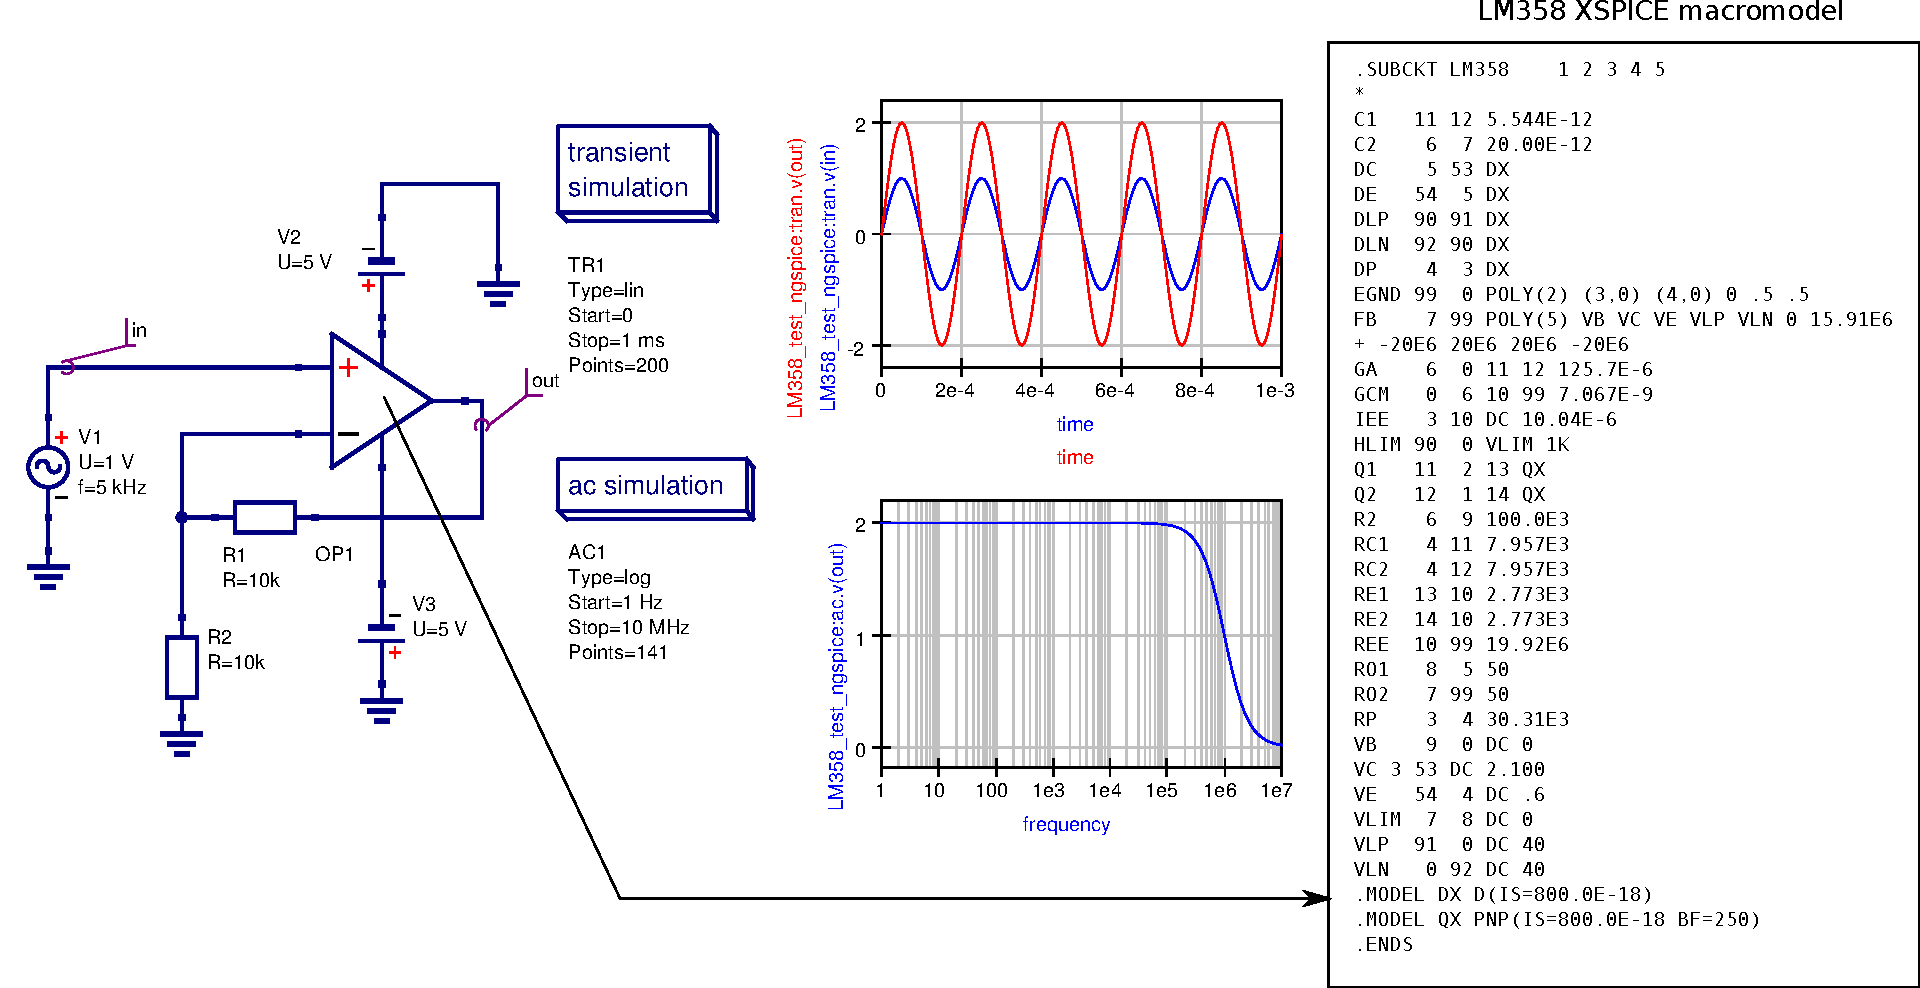
\includegraphics[width=\textwidth]{img/LM358.pdf}
 
 \end{frame}


\begin{frame}
 \frametitle{Compact modeling with Qucs and Ngspice/Xyce: Part VIII --- 
Capacitance probe usage for model parameters extraction}

\begin{itemize}
 \item Capacitance probe component (CMeter) introduced since 
Qucs-0.0.19
 \item It allows to extract capacitance of a circuit with Qucs and Ngspice
\end{itemize}

 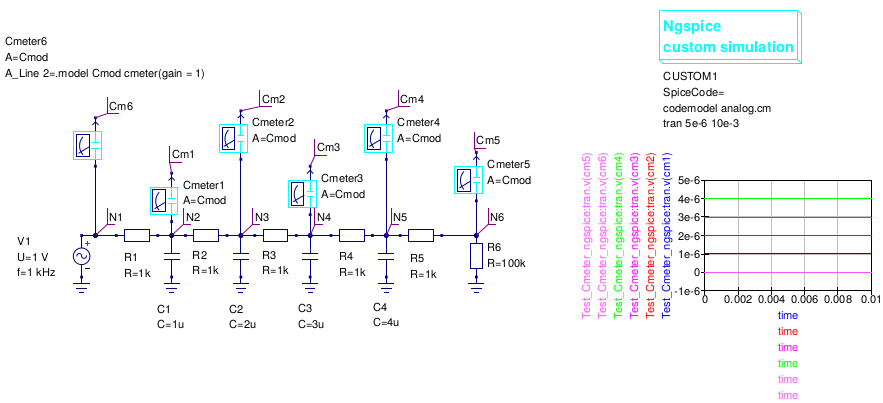
\includegraphics[width=\textwidth]{img/CMeter.png}

\end{frame}

\begin{frame}
 \frametitle{Overview of new components introduced in Qucs-0.0.19: Part I --- A 
short components list}

\begin{itemize}
 \item Spice specific components:
 \begin{itemize}
 \item Sources: B-type source, SPICE AC voltage source, SPICE noise sources;
 \item Modulated sources: AM, SFFM; 
 \item Piecewise source: PWL;
 \item Passive components: SPICE RCL, inductive coupling;
 \item Transmission lines: LTL, LTRA, UDRCTL;
 \item Semiconductor devices: diode, BJT, JFET, MOSFET, MESFET;
\end{itemize}
\item Spice netlist sections: .PARAM, .GLOBAL\_PARAM, .IC, .NODESET, .OPTIONS, 
Nutmeg equation
\item Spice specific simulations: .FOUR, .NOISE, .DISTO, Custom simulation
\end{itemize}


\end{frame}


\begin{frame}
  \frametitle{Overview of new components introduced in Qucs-0.0.19: \\ Part II 
--- New SPICE-compatible sources}

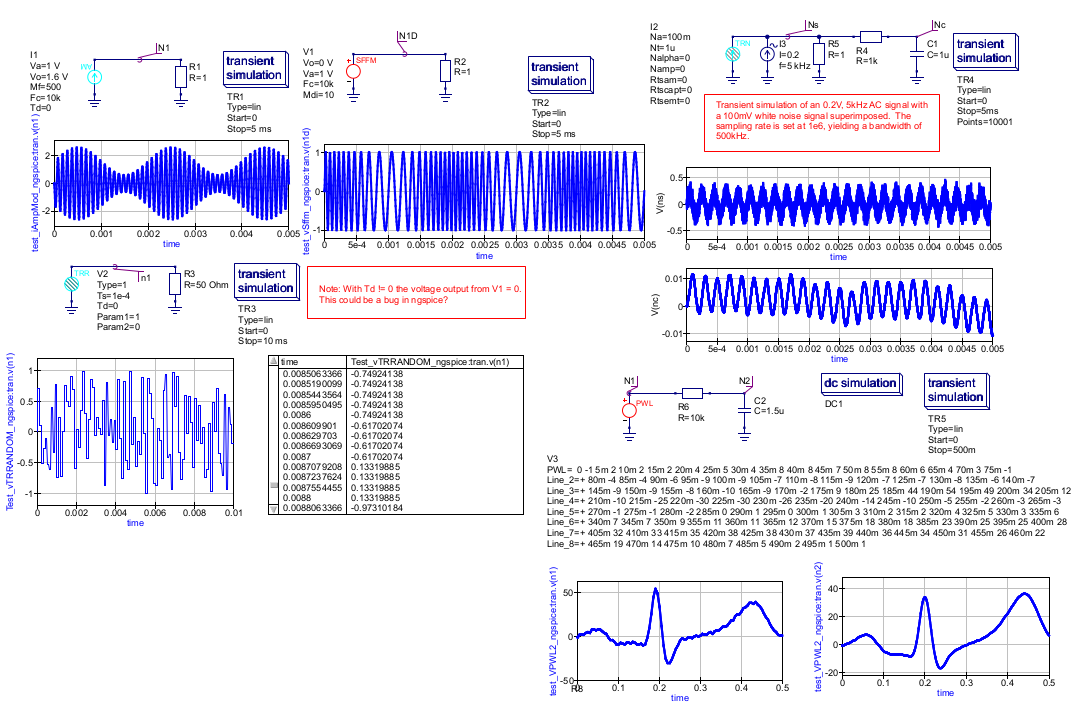
\includegraphics[width=\textwidth]{img/new_srcs.png}

\end{frame}

\begin{frame}
  \frametitle{Overview of new components introduced in Qucs-0.0.19: \\ Part IV 
--- New transmission lines models allow time-domain simulation}
  \centering
  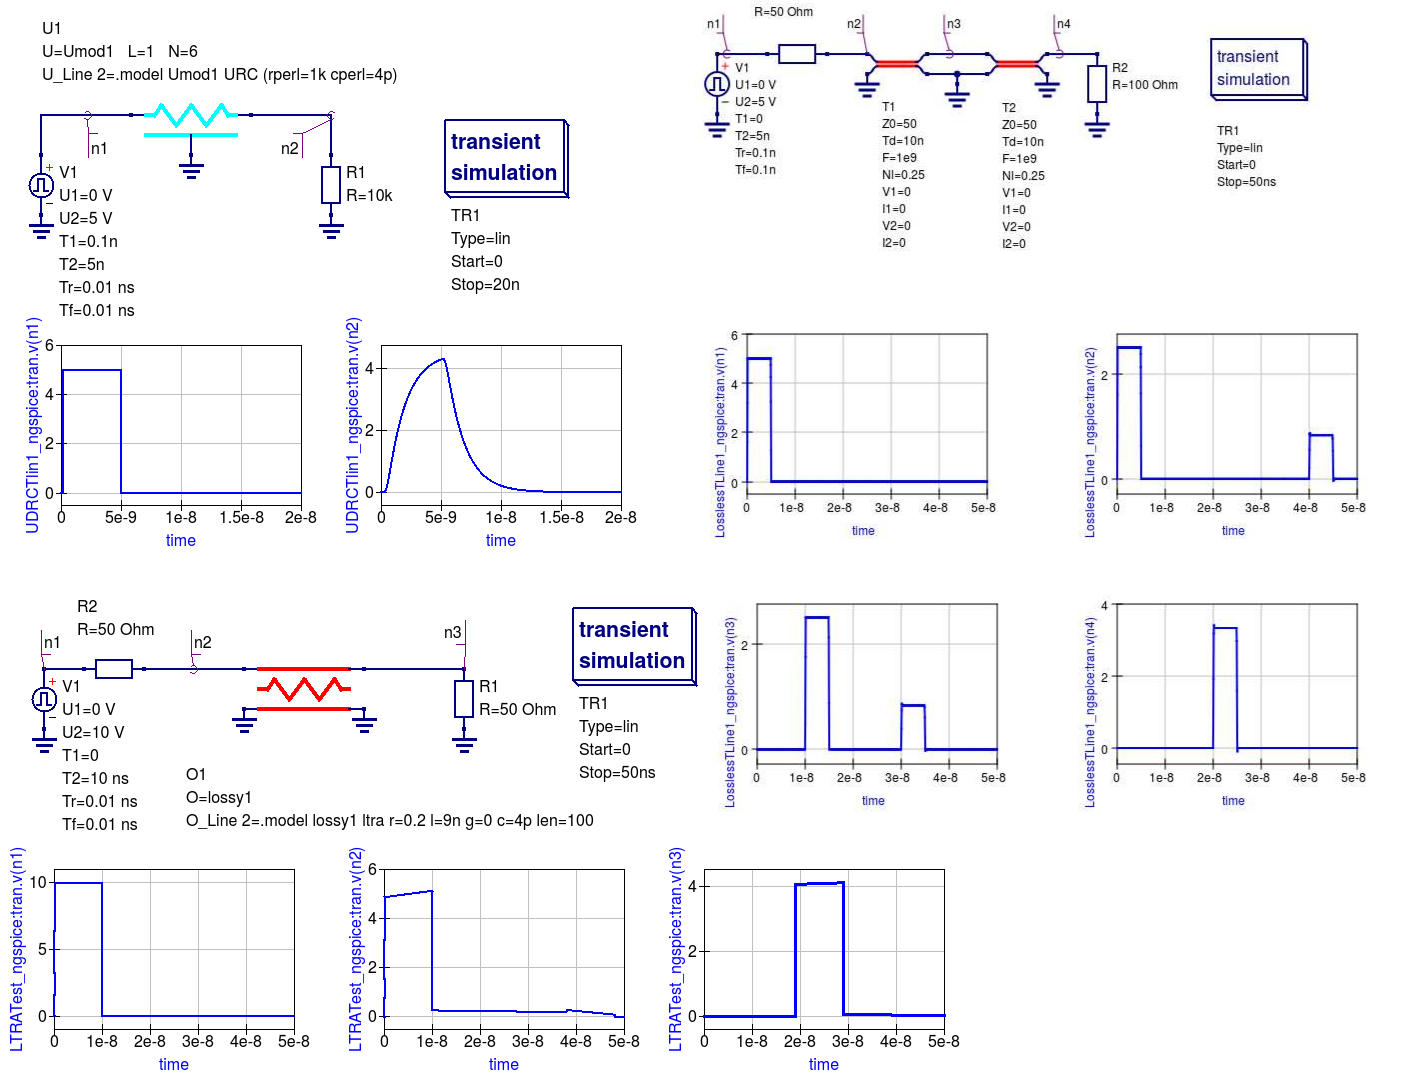
\includegraphics[width=0.8\textwidth]{img/tline.png}
\end{frame}

\begin{frame}
 \frametitle{Overview of new components introduced in Qucs-0.0.19: \\ Part IV 
--- Coupled inductors models}
 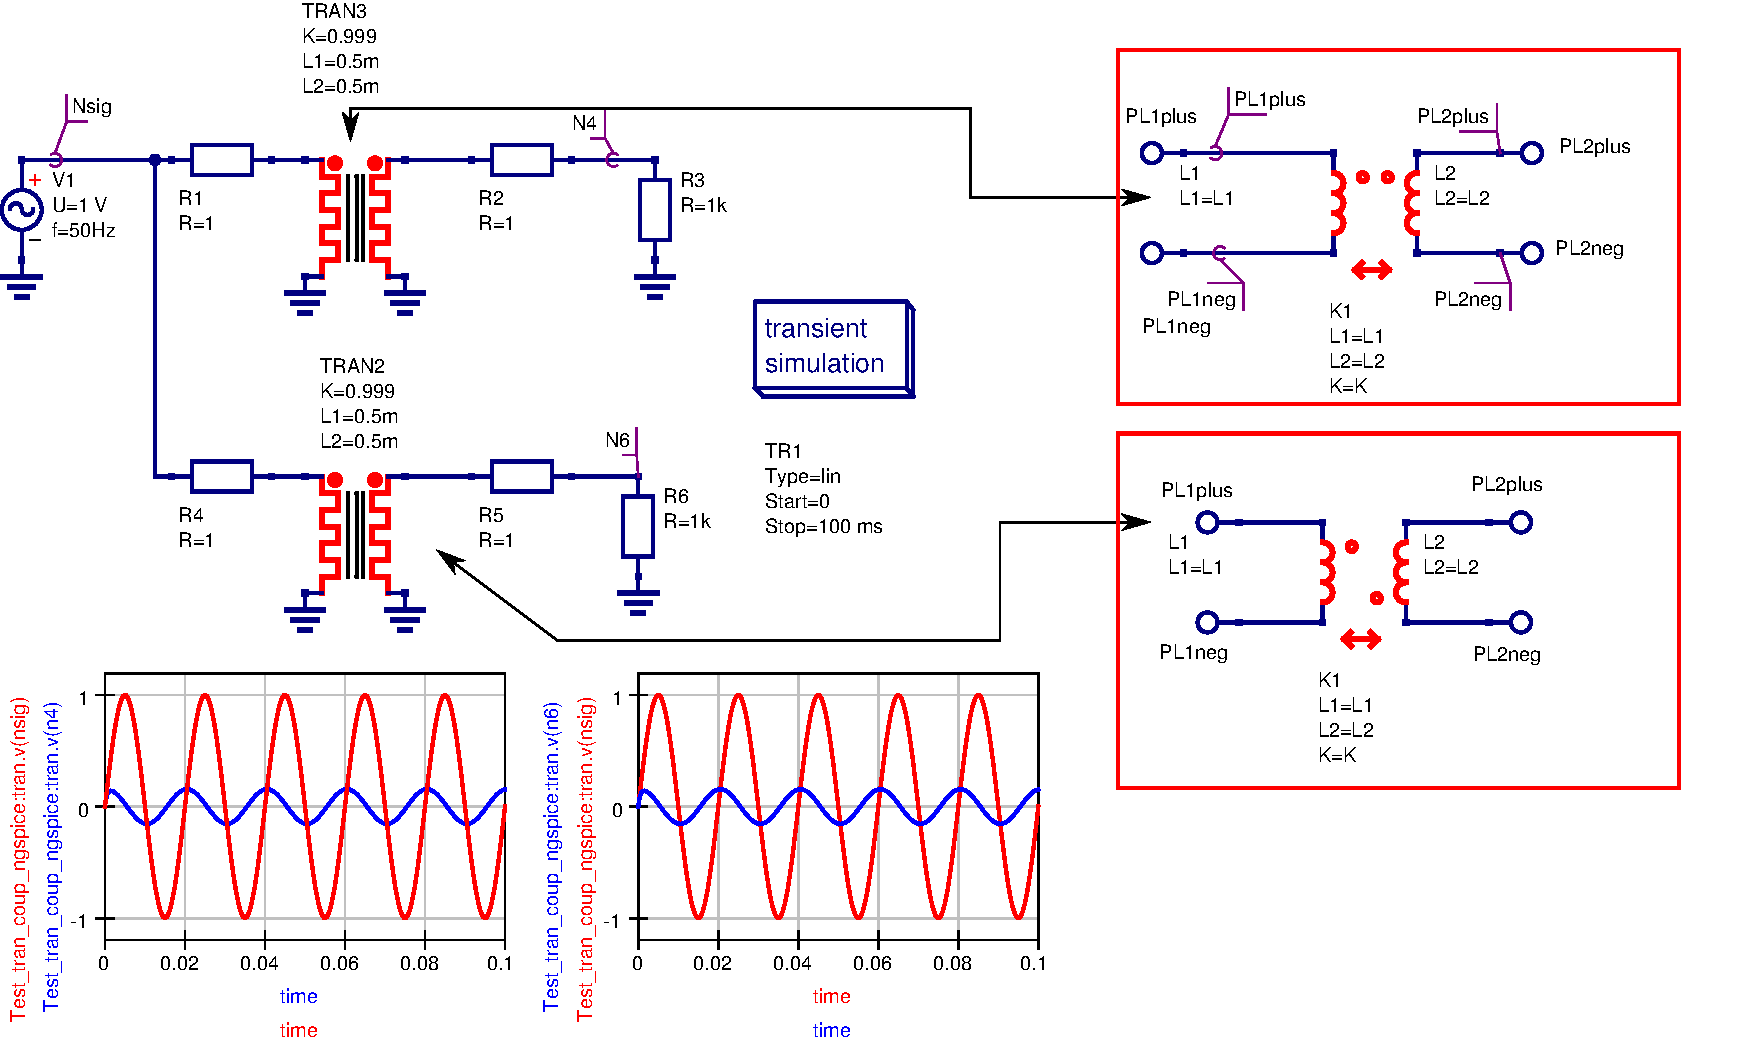
\includegraphics[width=\textwidth]{img/transf_test.pdf}
\end{frame}


\begin{frame}
  \frametitle{Overview of new components introduced in Qucs-0.0.19: \\ Part VI 
--- Semiconductor devices with full SPICE definition}
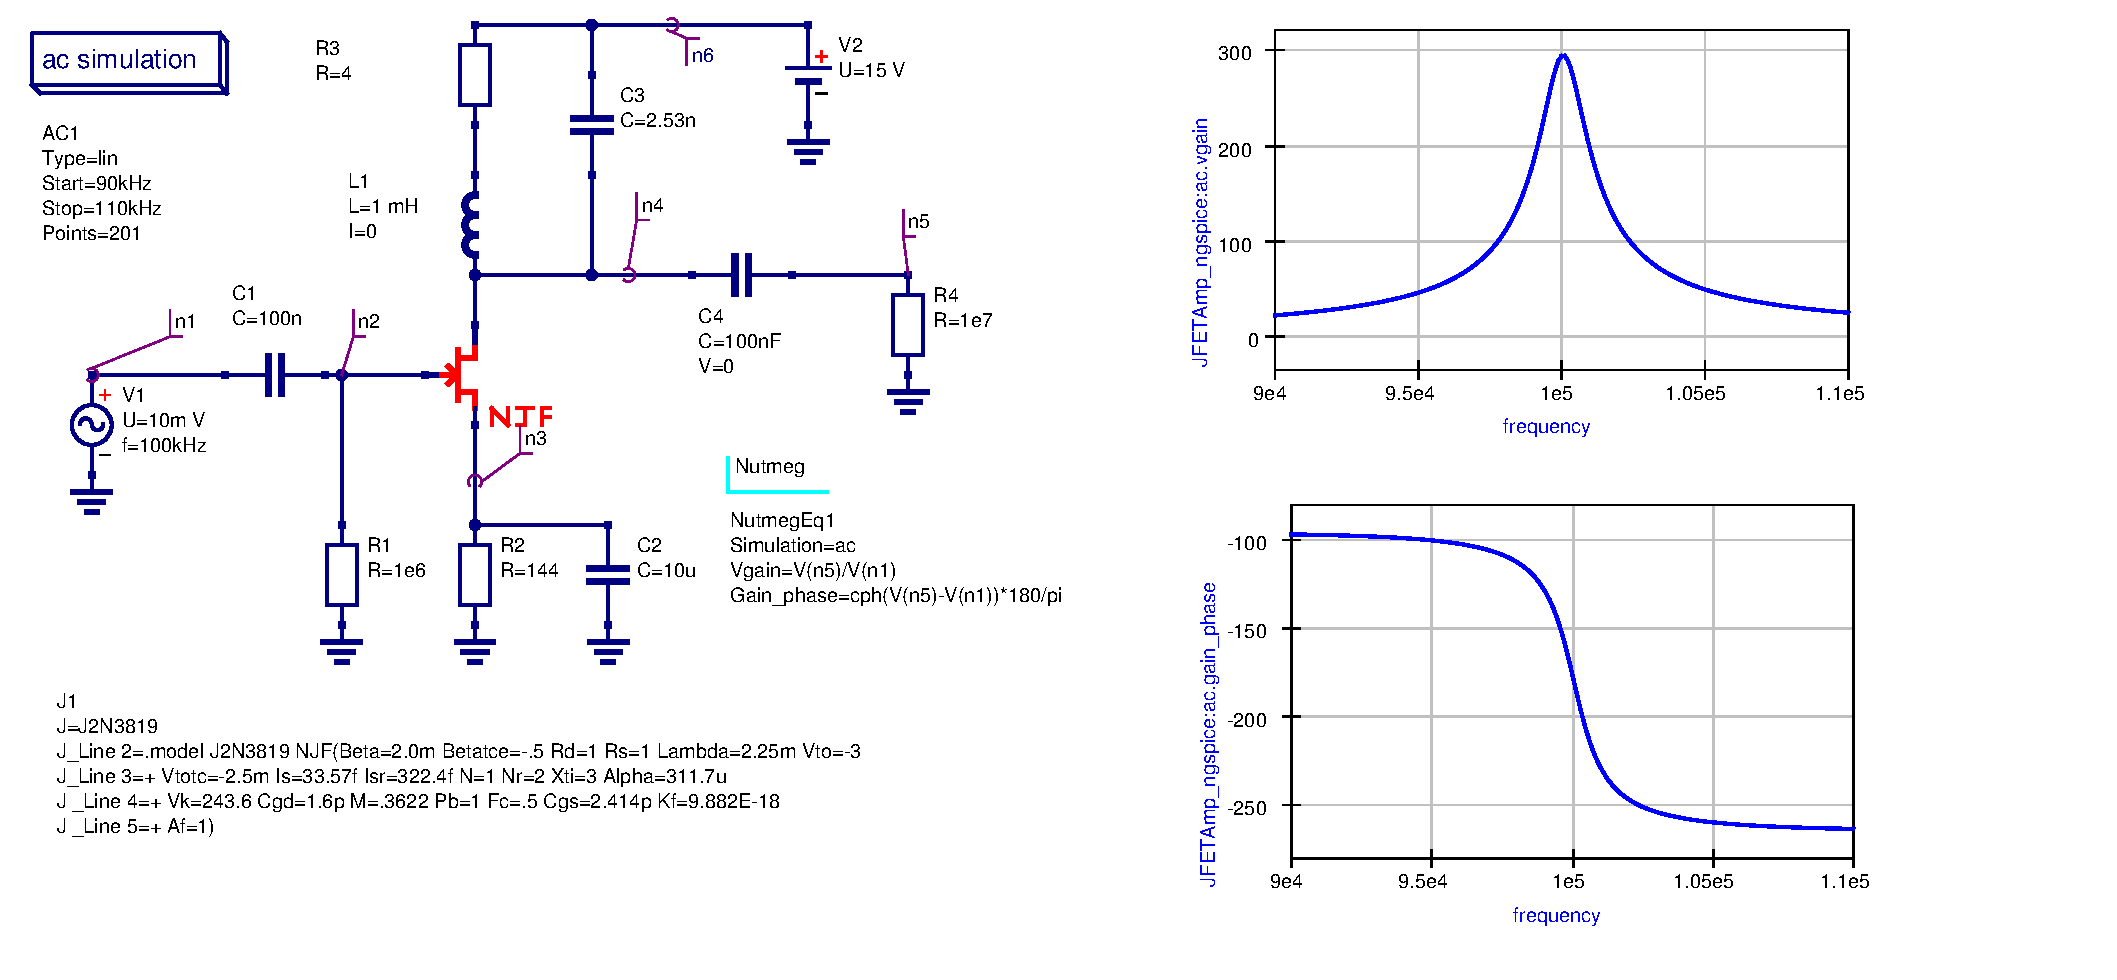
\includegraphics[width=1.2\textwidth]{img/njfet.pdf}
\end{frame}


\begin{frame}
 \frametitle{Qucs equations support in Spice4qucs}
 
 Let's evaluate the total $S$, active $P$, and reactive $Q$ power of an 
RC-circuit:

\begin{equation}
 S = abs (U \cdot \bar{I}) \qquad P = \Re [U \cdot \bar{I}]
 \qquad Q = \Im [U \cdot \bar{I}]
\end{equation}

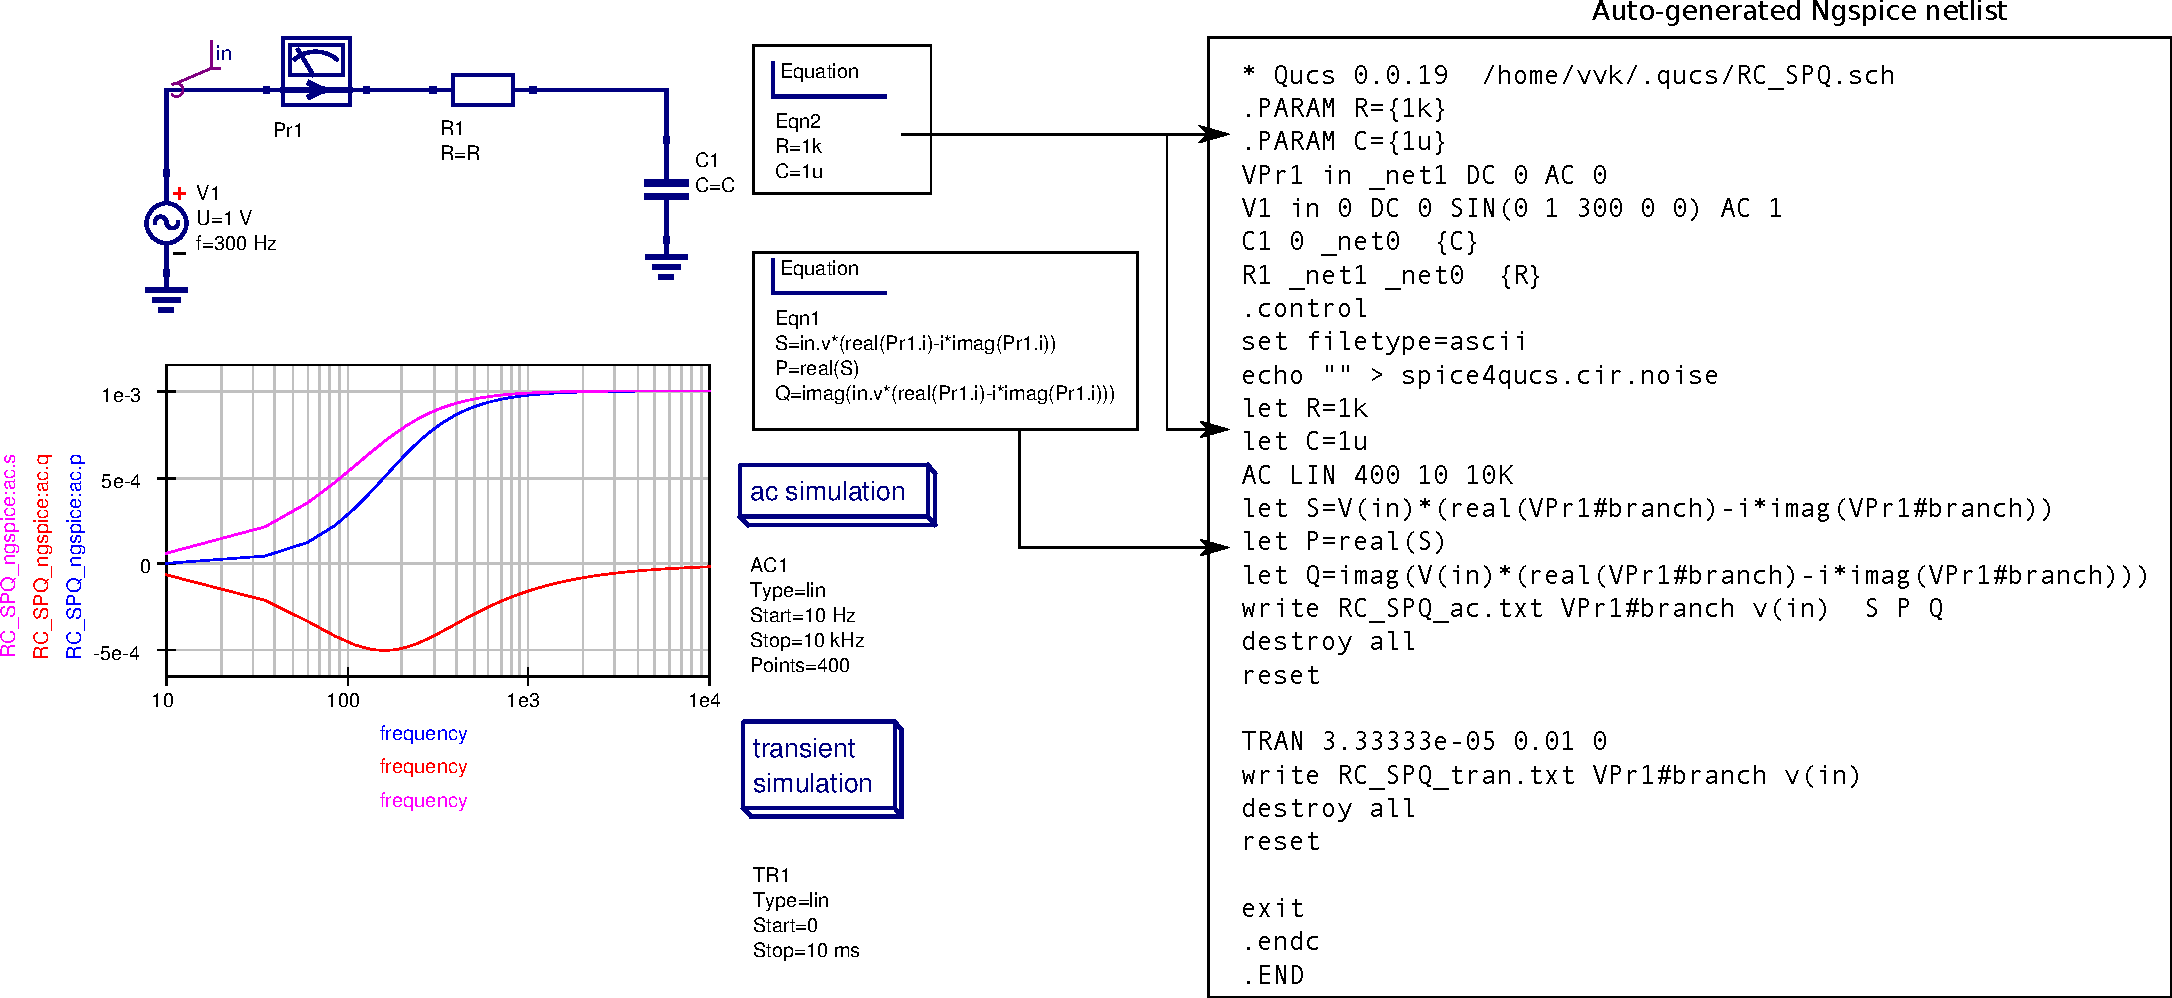
\includegraphics[width=1.05\textwidth]{img/RC_SPQ.pdf}

    
\end{frame}


\begin{frame}
 \frametitle{SPICE-style parametrization and Nutmeg postprocessor usage with 
Spice4qucs}

The following components serve for parametrization and postprocessing:
\begin{itemize}
 \item SPICE .PARAM section
 \item Nutmeg equation
\end{itemize}


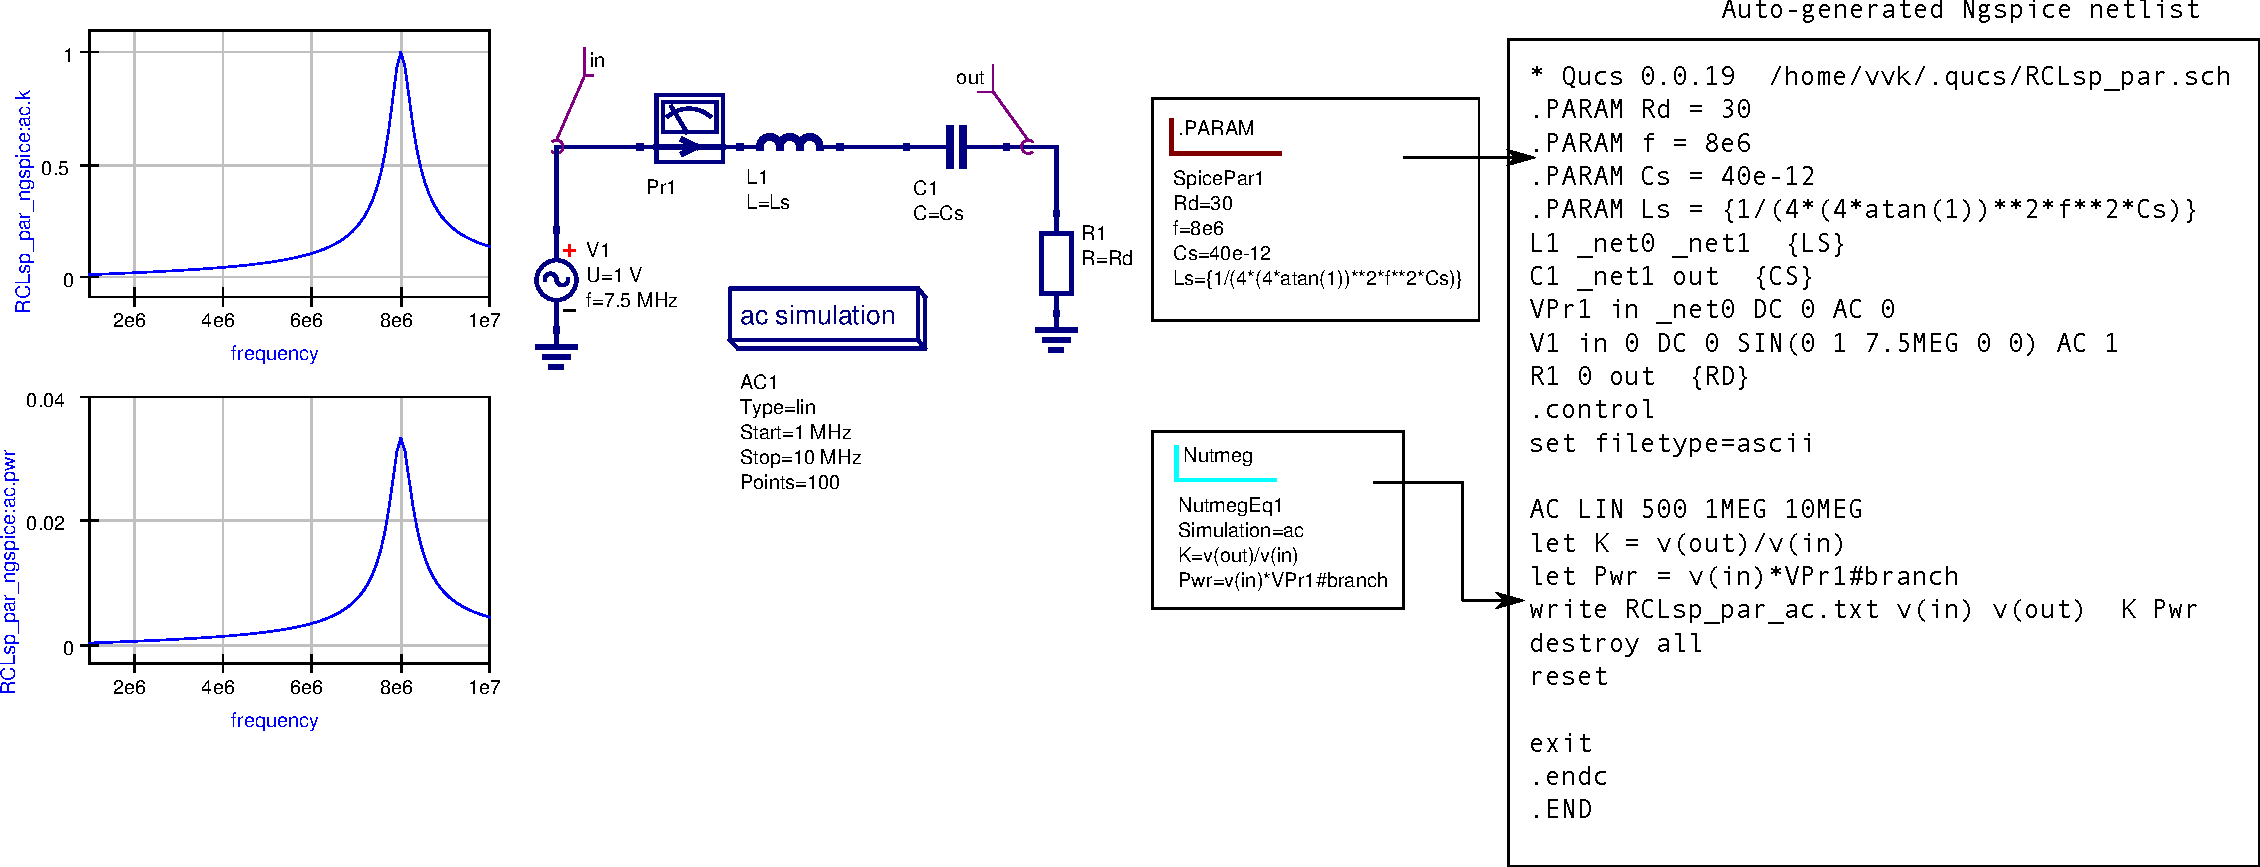
\includegraphics[width=1.05\textwidth]{img/RCLp.pdf}
\end{frame}

\begin{frame}
 \frametitle{New analysis types with spice4qucs: \\
 Small signal distortion, noise, and Fourier}
\centering
\mbox{}\hspace{1.5cm}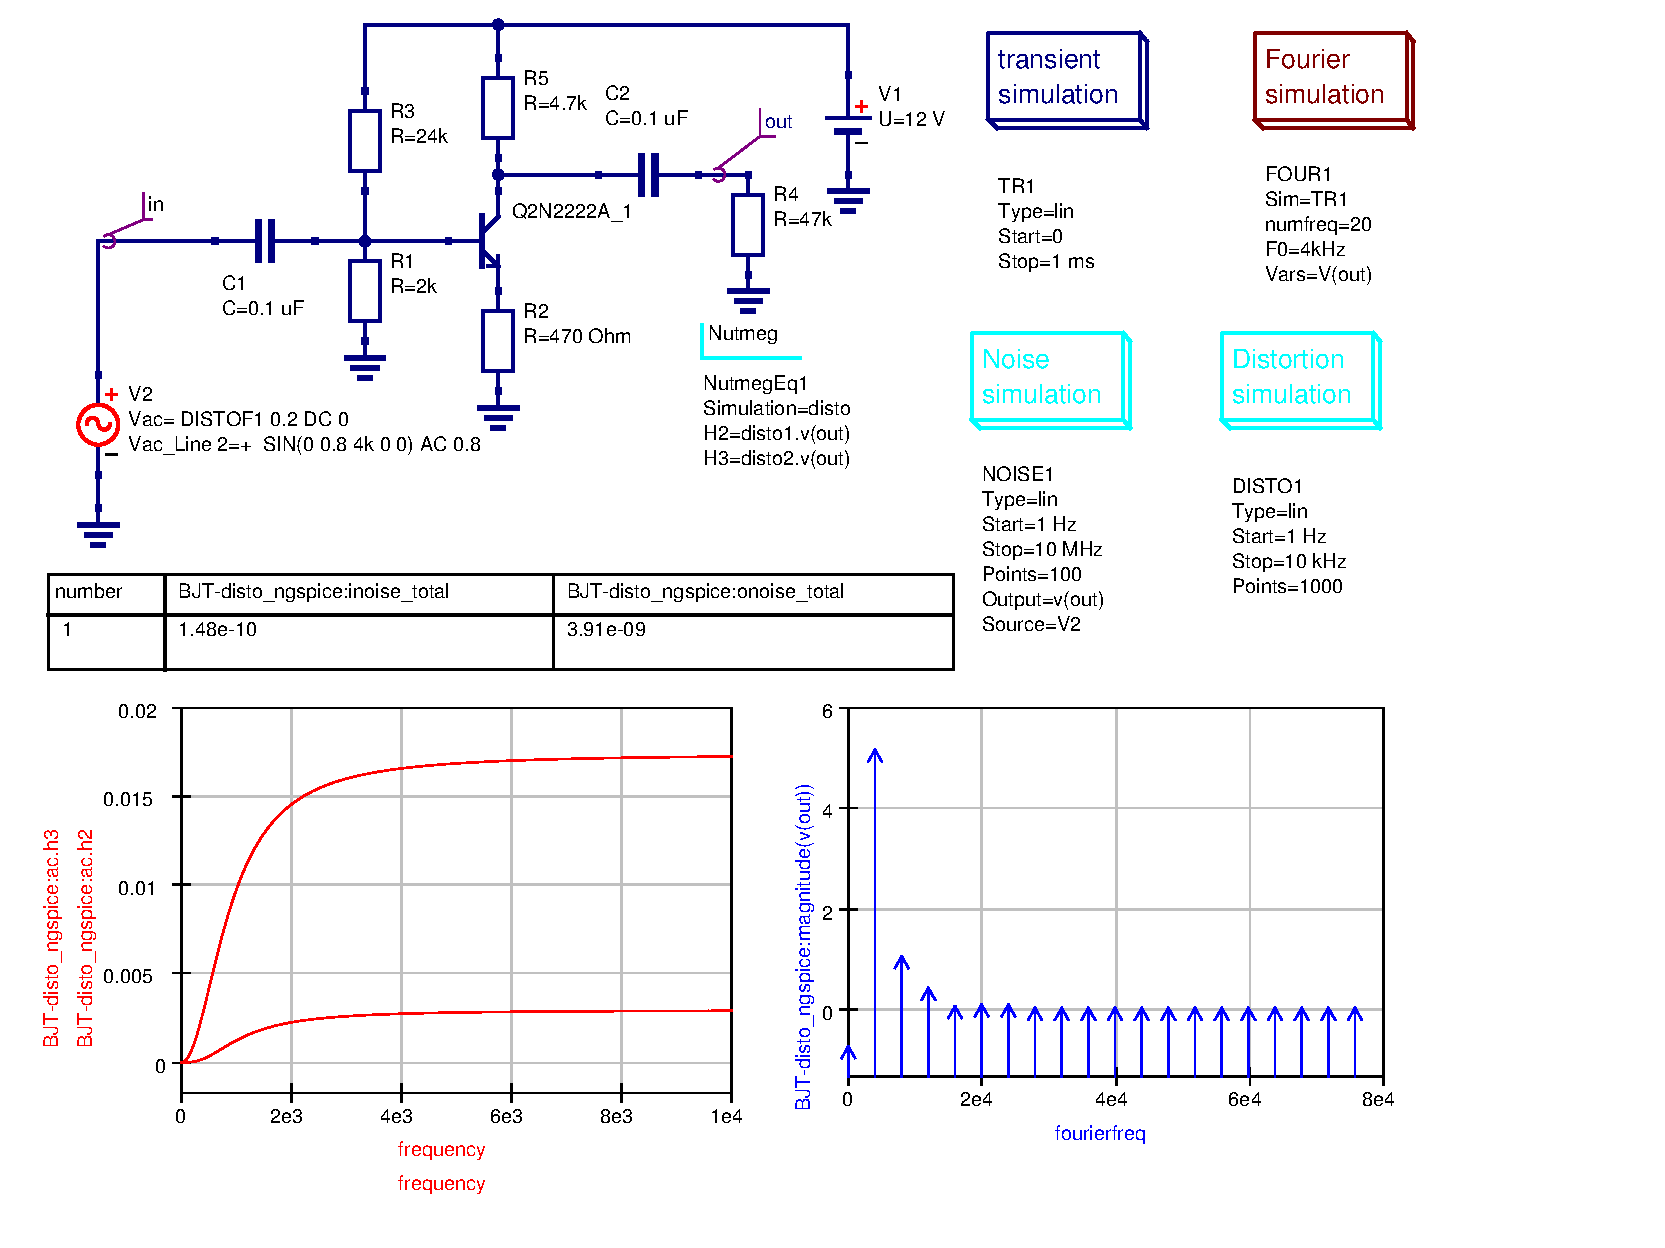
\includegraphics[width=0.95\textwidth]{img/BJT-disto.pdf}
\end{frame}


\begin{frame}
 \frametitle{Ngspice custom simulation technique: Part I --- Main features}
 
   \begin{tabular}{p{0.4\textwidth}p{0.6\textwidth}}
   Main features:
   \begin{itemize}
    \item Embedding user-defined ngnutmeg script in Qucs schematic
    \item Full Ngnutmeg support
    \item User-defined variables for plotting
    \item User-defined raw ASCII SPIE3f5 outputs to parse 
   \end{itemize}

    & 
    \begin{itemize}
     \item Ngnutmeg script edit dialog
    \end{itemize}
    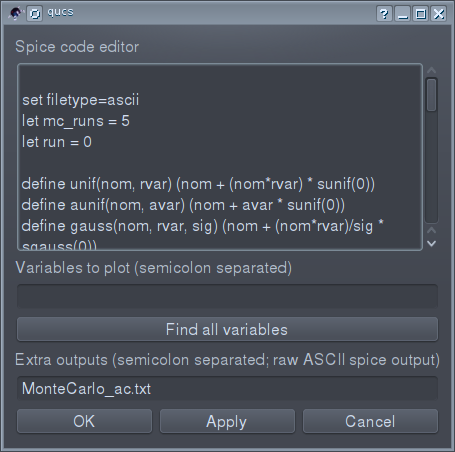
\includegraphics[width=0.6\textwidth]{img/customsim_dlg}
    
    \\
   \end{tabular}

\end{frame}

\begin{frame}
 \frametitle{Ngspice custom simulation technique: Part II --- Application 
example: Monte-Carlo simulation with Ngnutmeg script}

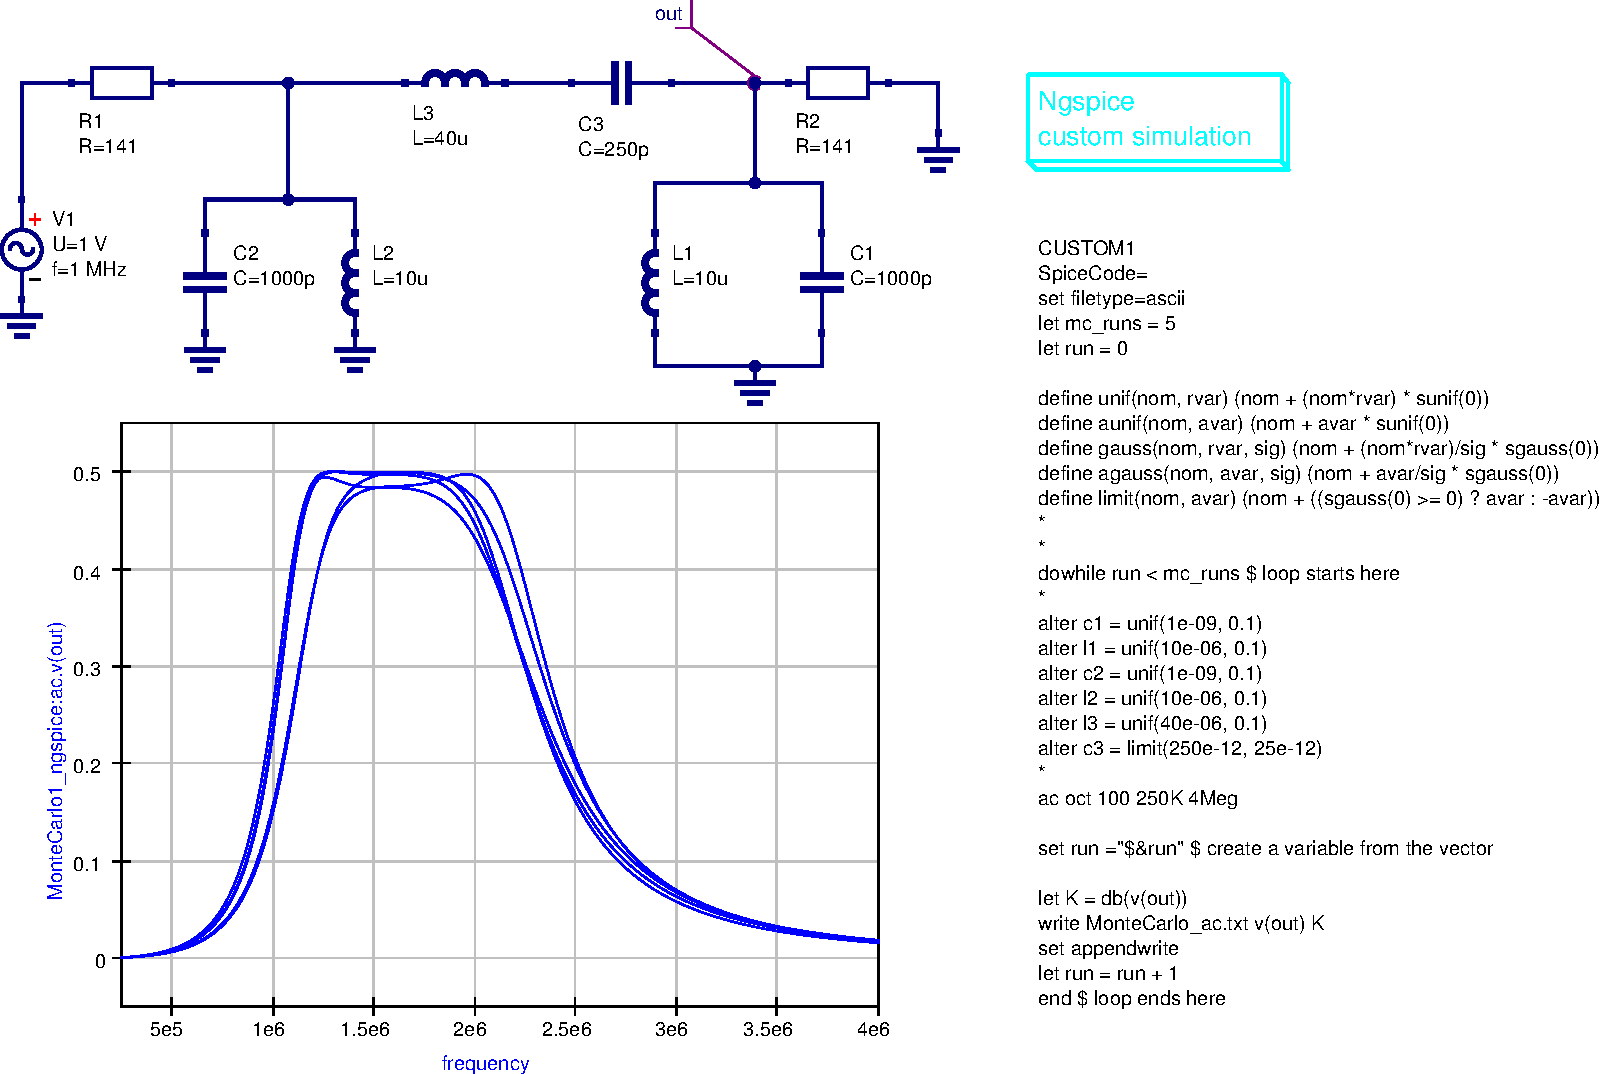
\includegraphics[width=0.95\textwidth]{img/monte-carlo.pdf}
\end{frame}

\begin{frame}
 \frametitle{Extended passive filter synthesis tool Qucsfilter}
 
 \begin{tabular}{p{0.3\textwidth}p{0.7\textwidth}}
  
  Filter topologies added in Qucs-0.0.19:
  
  \begin{itemize}
   \item C-coupled transmission lines
   \item Coupled microstrip
   \item Coupled transmission lines
   \item End-coupled microstrip
   \item Stepped impedance
   \item Stepped impedance microstrip
  \end{itemize}

  
  & \begin{itemize}
     \item Qucsfilter utility main window
    \end{itemize}
    
    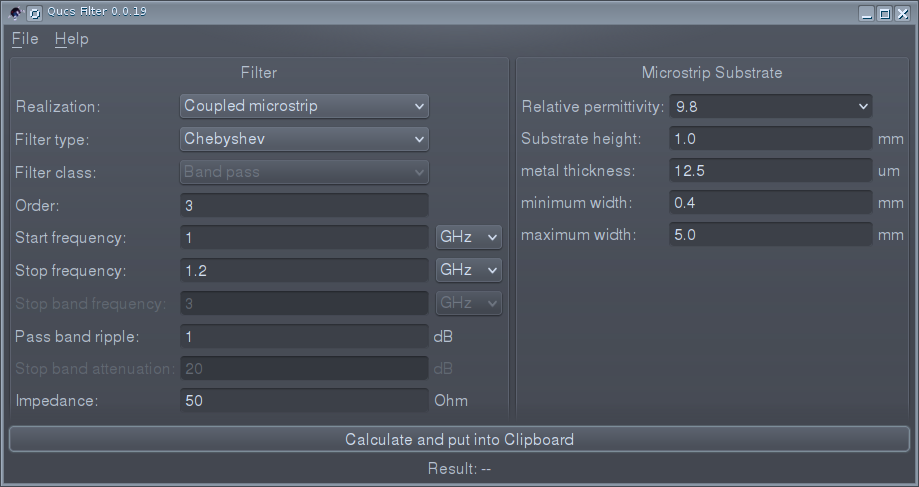
\includegraphics[width=0.7\textwidth]{img/passivefilt.png}
    
    \begin{itemize}
     \item To be released with 0.0.19
    \end{itemize}

\\
 \end{tabular}
 
\end{frame}

\begin{frame}
 \frametitle{Auto-synthesized microstrip filter topology and its magnitude 
response}
 
 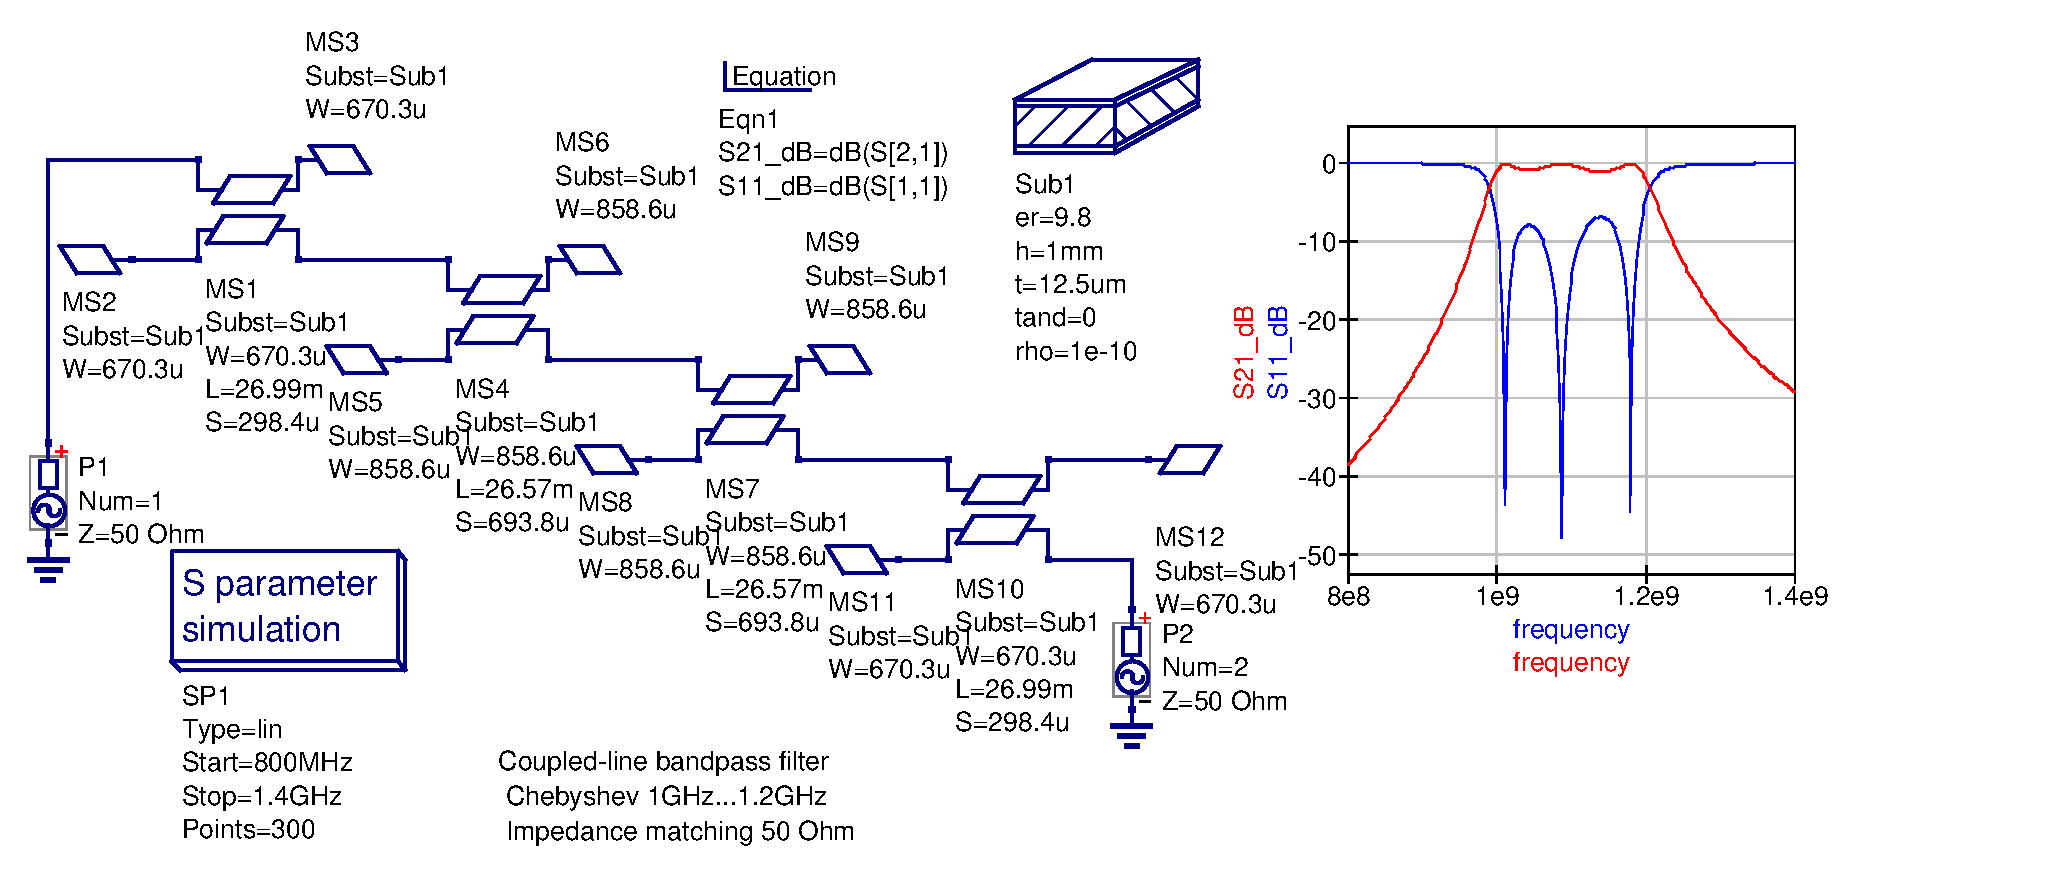
\includegraphics[width=1.1\textwidth]{img/msfilt.pdf}
\end{frame}
 

\begin{frame}
 \frametitle{A new utility for Active filter synthesis}
%  \centering
\begin{tabular}{p{0.35\textwidth}p{0.65\textwidth}}
\small
 Main features 
 \begin{itemize}
  \item Butterworth, Chebyshev (Type I and II), Bessel, and Cauer low-pass, 
high-pass, band-pass, and band-stop active filters design
  \item Sallen-Key, Multifeedback, and Cauer filter section topologies are 
available.
  \item User-defined filter transfer functions
  \item Full Qucs integration. Copy-paste interface with Qucs.
  \item Coming soon with 0.0.19 release
 \end{itemize}
 &

 Main window of Qucsactivefilter
 
  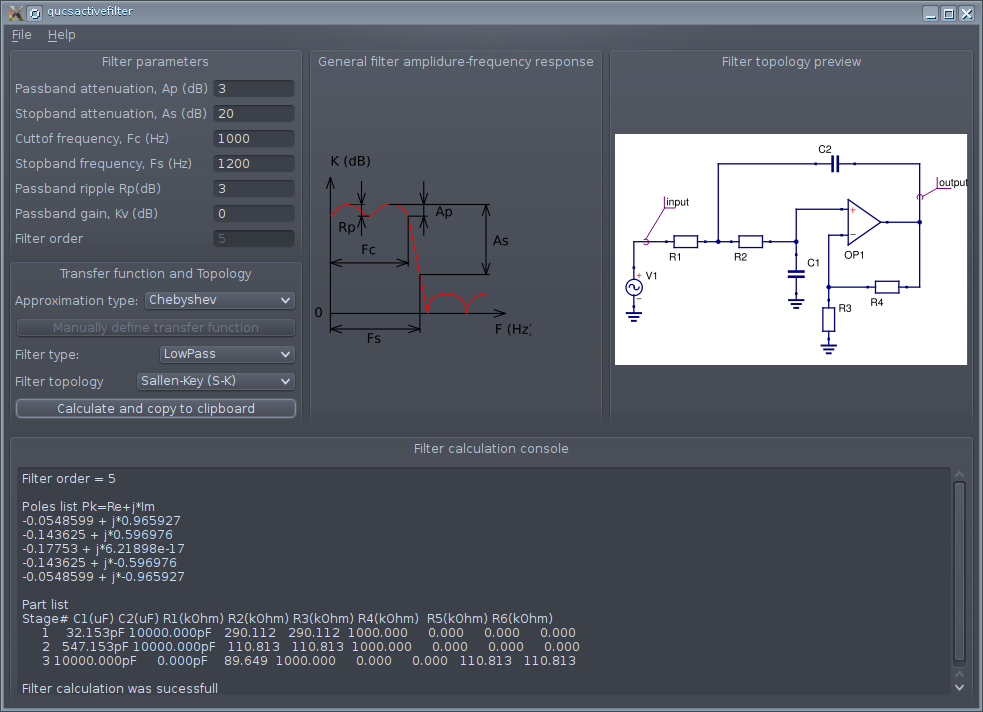
\includegraphics[width=0.65\columnwidth]{img/actfilt-win.png}
 \\
\end{tabular}
\end{frame}


\begin{frame}
 \frametitle{Auto-synthesized Chebyshev 5th-order filter  and its 
magnitude response}
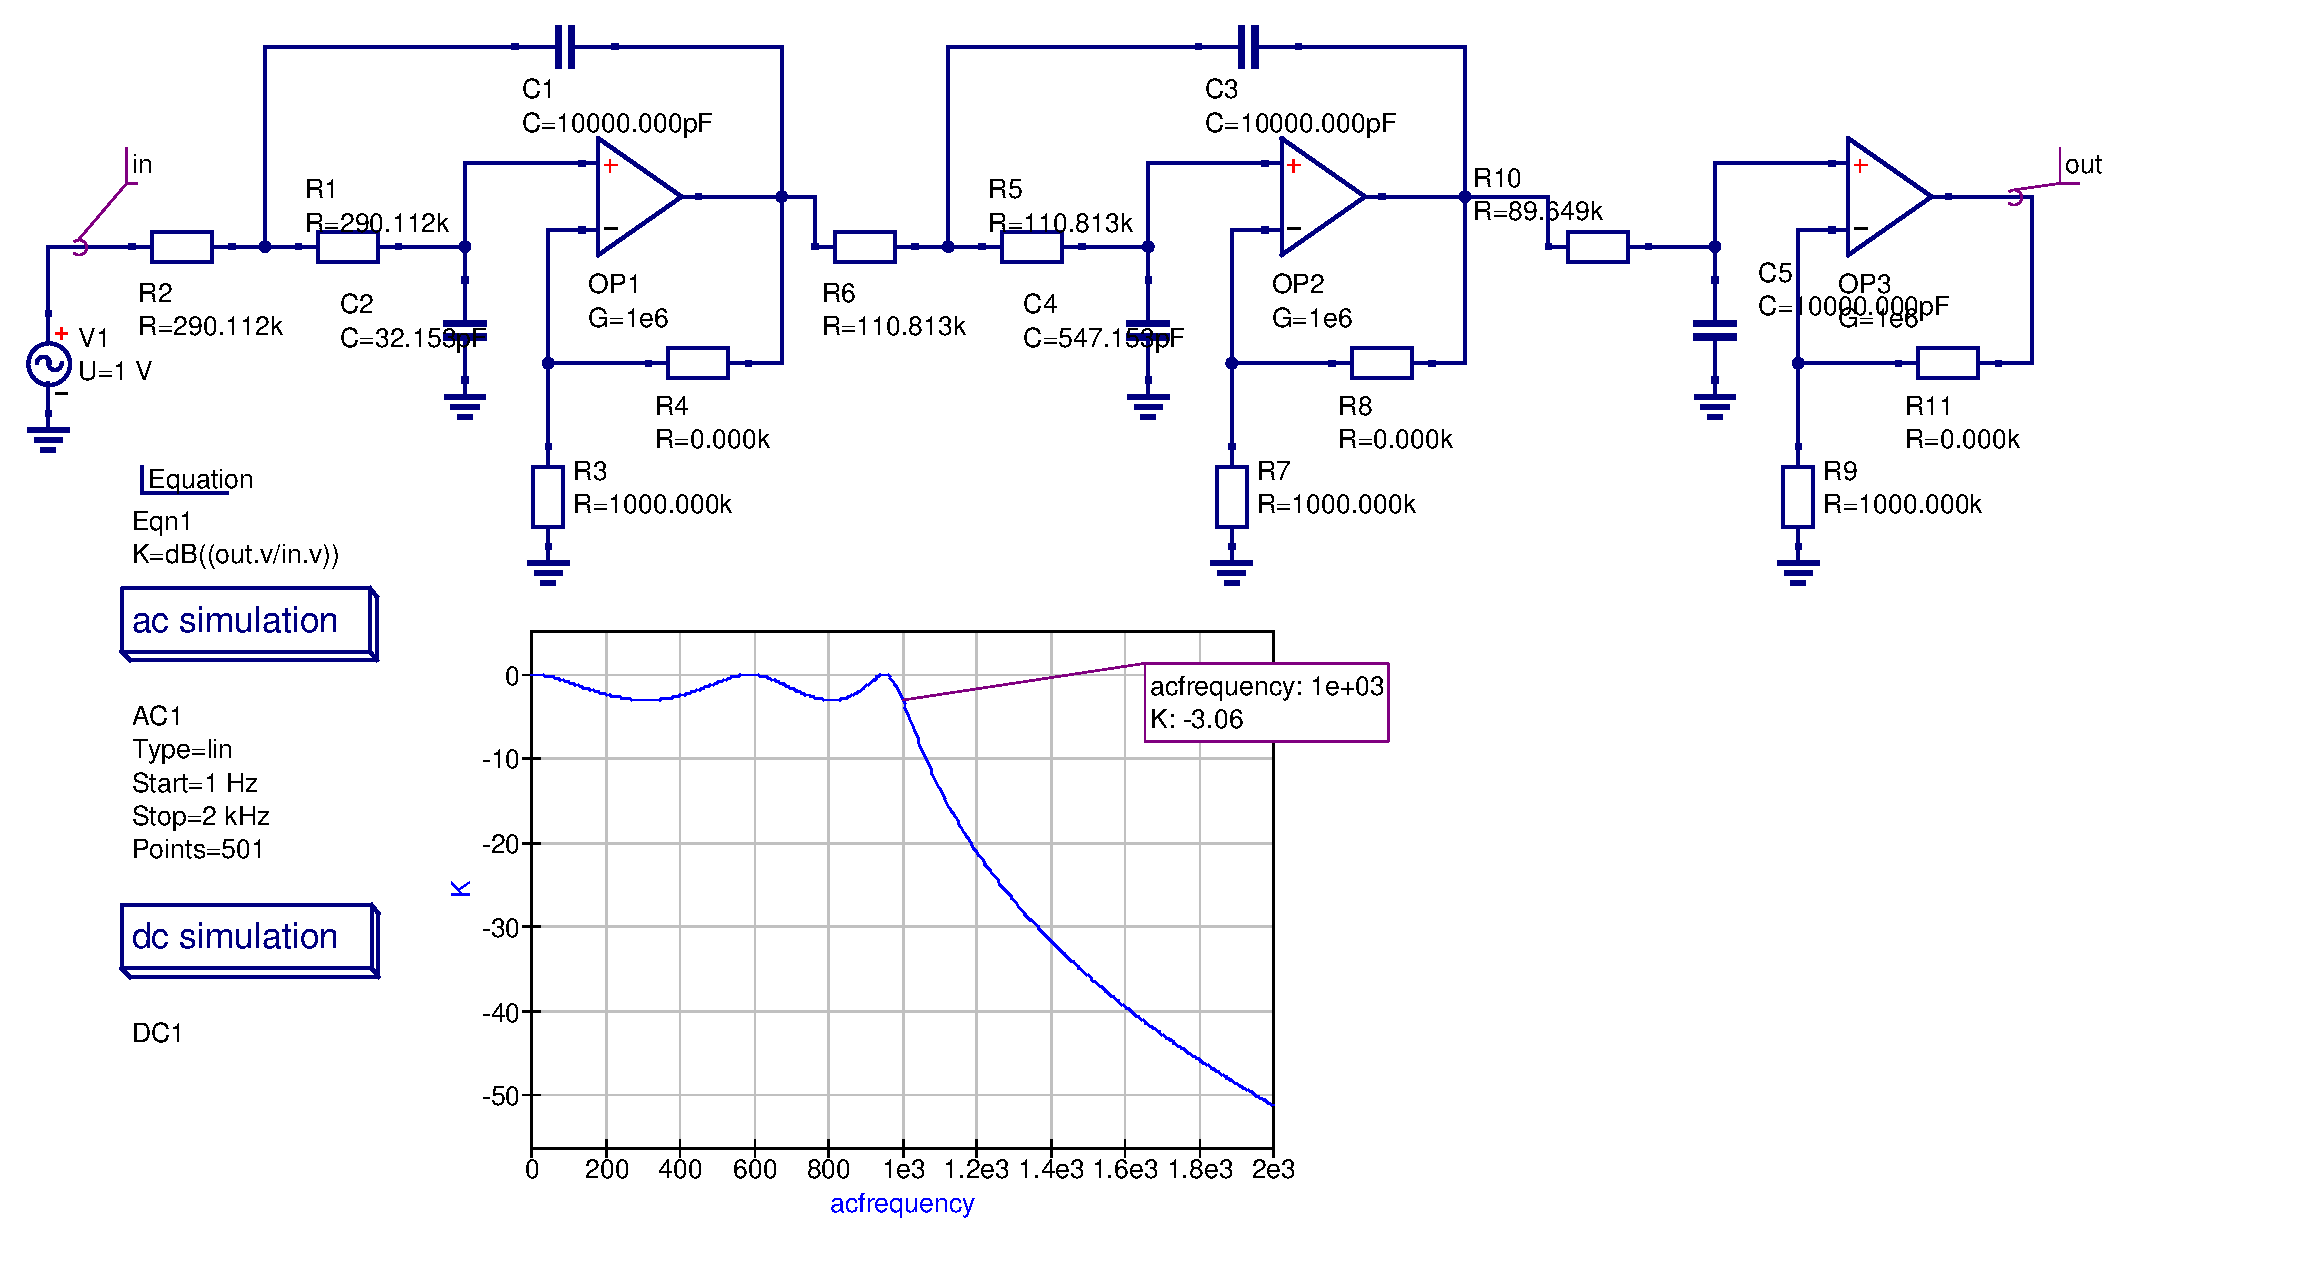
\includegraphics[width=1.1\textwidth]{img/actfilt.pdf}
\end{frame}



\begin{frame}
 \frametitle{Verilog-A modules building from EDDs concept}

   \begin{tabular}{p{0.4\textwidth}p{0.6\textwidth}}
Future Verilog-A module builder allows you to "close loop", i.e to build new 
component from mathematical model performing the following steps:
\begin{itemize}
 \item Build EDD from mathematical model
 \item Test EDD with Qucsator, Ngspice, and Xyce
 \item Build Verilog-A module from EDDs
 \item Build C++ source file from Verilog-A using ADMS
 \item Embed new component in Qucs
\end{itemize}

 & \begin{itemize}
    \item Component build workflow:
   \end{itemize}
   
   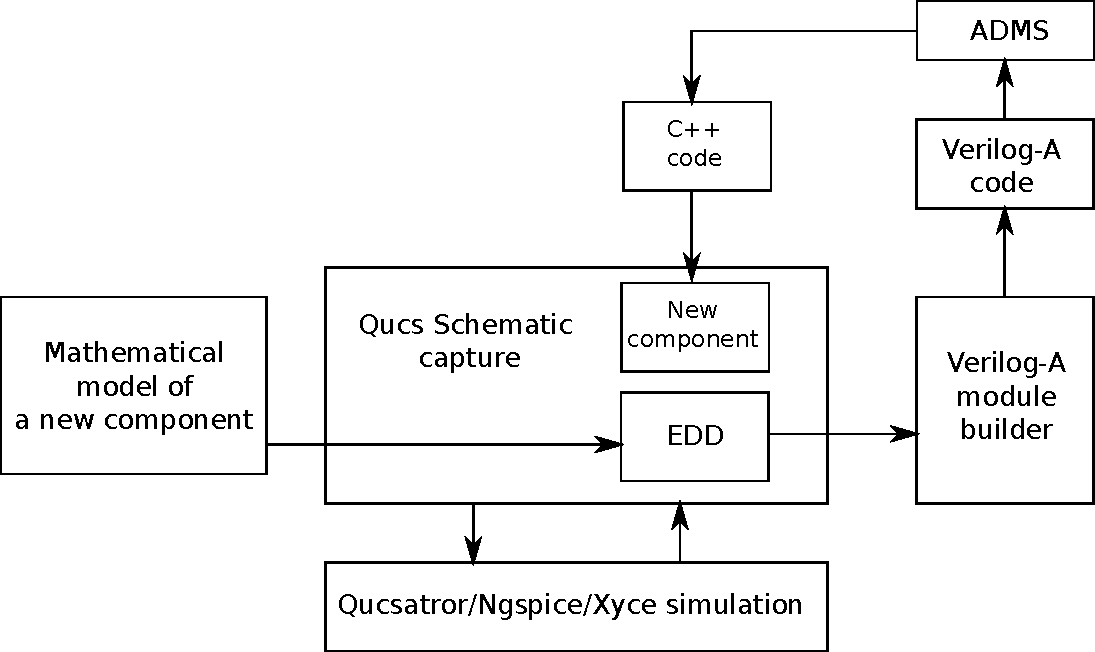
\includegraphics[width=0.5\textwidth]{img/verilogA.pdf}
 \\
\end{tabular}




\end{frame}

\begin{frame}
 \frametitle{RFEDD support in spice4qucs: Part I --- The problem}

\begin{itemize}
 \item Let's consider an inductor with frequency-dependent losses
 
 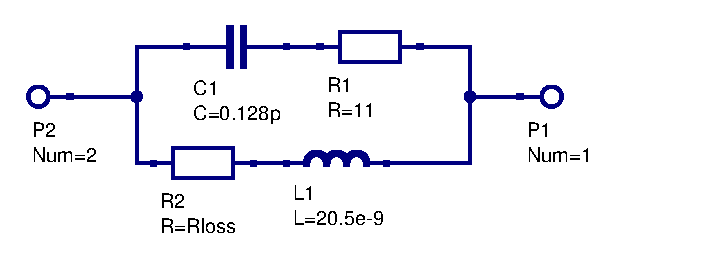
\includegraphics[width=7cm]{img/lossL.pdf}
 
 \item Losses resistance frequency dependency
 \begin{equation}
  R_{loss}(f) = K_1 \sqrt{F}
 \end{equation}
 \item Equivalent Z-parameters matrix:
 \begin{equation}
  Z = \left[
  \begin{matrix}1 & K_1\sqrt{F} \\ 1 & 0 \end{matrix}
  \,\right]
 \end{equation}

\end{itemize}

\end{frame}

\begin{frame}
\frametitle{RFEDD support in spice4qucs: Part II --- Ngspice approach}


\begin{itemize}
 \item SPICE system hertz variable could be used in expressions to represent 
frequency-dependent passive (RCL) component
\end{itemize}

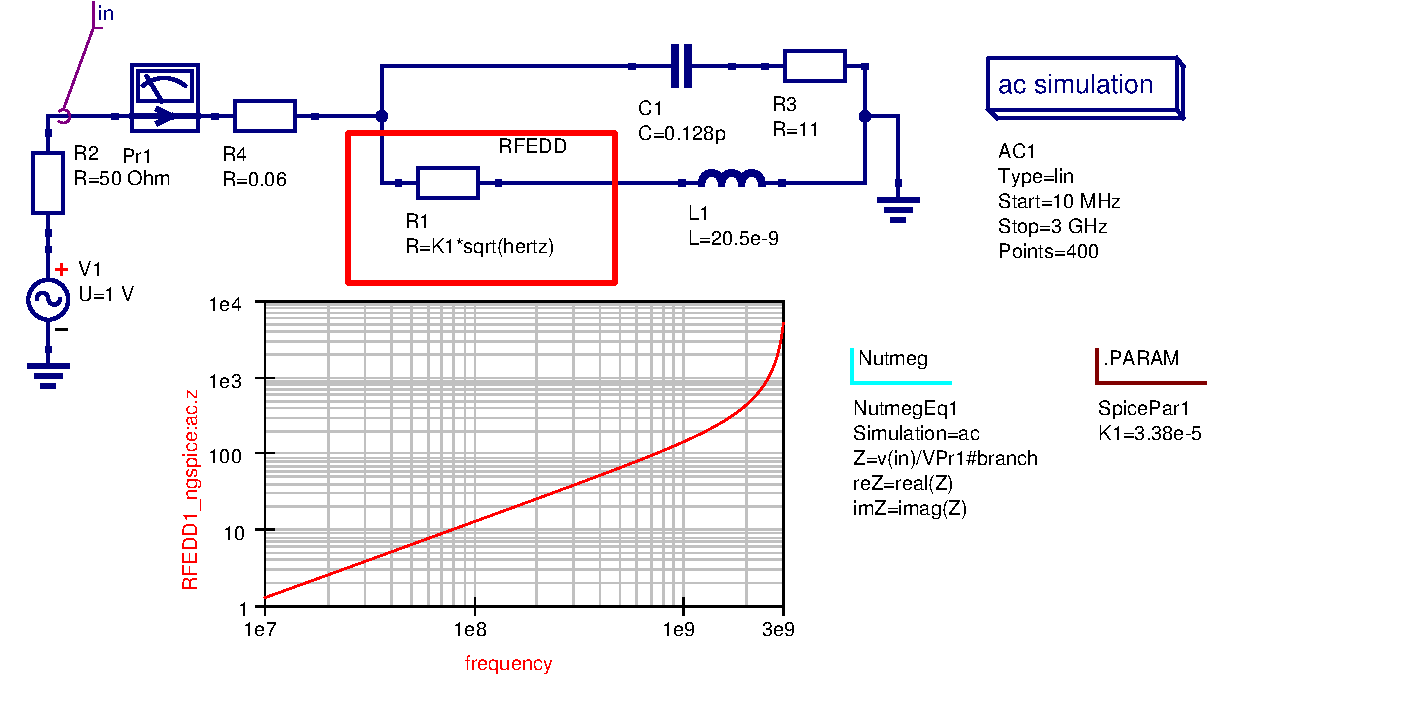
\includegraphics[width=1.1\textwidth]{img/RFEDDsp.pdf}
\end{frame}

\begin{frame}
\frametitle{RFEDD support in spice4qucs: Part III --- Qucs RFEDD equivalent 
circuit}
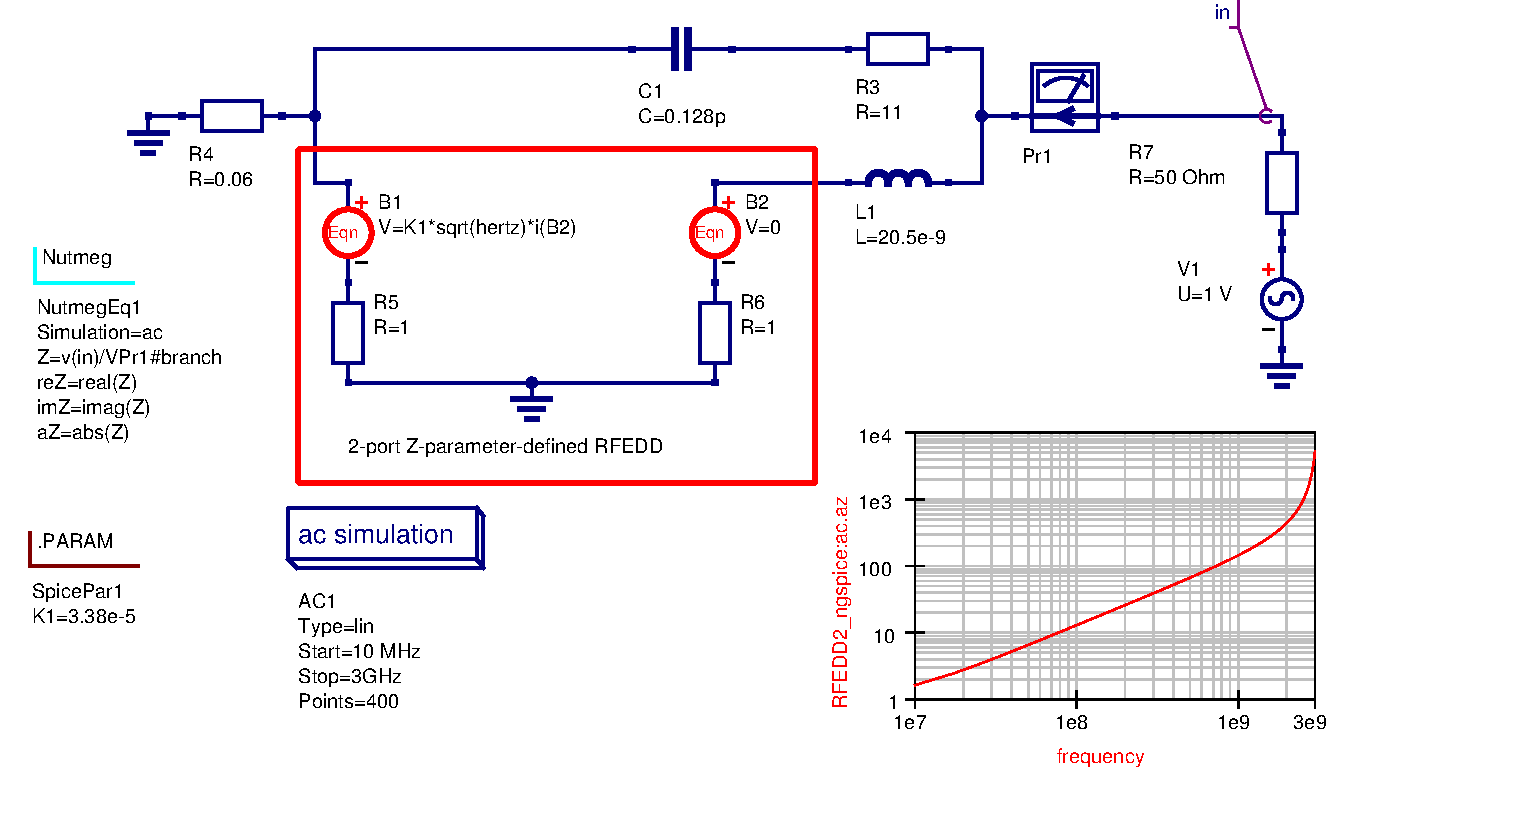
\includegraphics[width=1.1\textwidth]{img/RFEDD2p.pdf}
\end{frame}

\begin{frame}
 \frametitle{Gnucap as simulation backend}
 \begin{itemize}
  \item Patch by Felix Salfelder allows you to use Gnucap as simulation backend 
for Qucs GUI
  \item Source code and initial documentation available at 
\url{http://git.savannah.gnu.org/cgit/gnucap/gnucap-plugins.git/log/?h=qucs}
  \item This circuit is simulated with Gnucap.
 \end{itemize}
 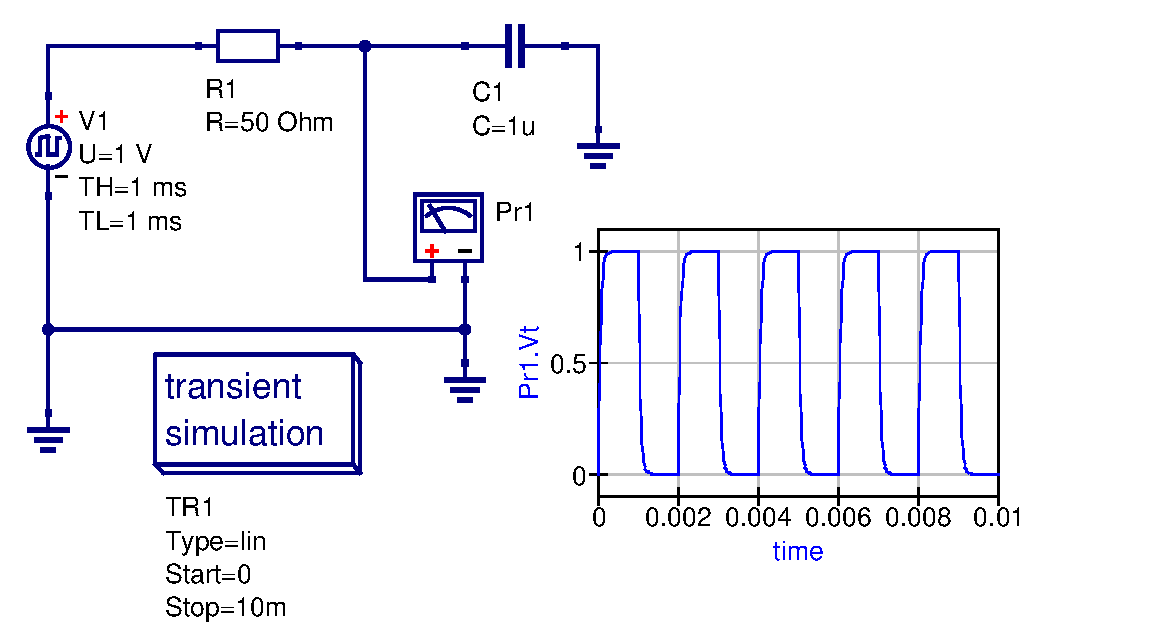
\includegraphics[width=0.8\textwidth]{img/gnucap.pdf}
 
\end{frame}


\begin{frame}
 \frametitle{Conclusion}
 
 Summary and possible future development directions:

 \begin{itemize}
  \item Qucs 0.0.19 is likely to be a major release of the circuit simulator 
package with many of the features introduced in this presentation included. The 
main development directions will be following
  \item Further integration with Ngspice and Xyce: improvement of Nutmeg 
support, RFEDD implementation, additional analysis support (.SENS and .PZ), 
new SPICE-compatible components (magnetic cores, etc.).
  \item EDDs to Verilog-A modules converter implementation.
  \item Mixed signal simulation with Ngspice (via XSPICE) implementation.
  \item Gnucap simulation backend support (by Felix Salfelder). 
  \item  Revised Qucs Wiki roadmap can be found at 
\url{https://github.com/Qucs/qucs/wiki/Roadmap}

 \end{itemize}

 
\end{frame}


\end{document}
